\documentclass[
	%parspace, % Add vertical space between paragraphs
	%noindent, % No indentation of first lines in each paragraph
	%nohyp, % No hyphenation of words
	%twoside, % Double sided format
	%draft, % Quicker draft compilation without rendering images
	%final, % Set final to hide todos
]{elteikthesis}[2024/04/26]

% The minted package is also supported for source highlighting
% See elteikthesis_minted.tex for example
%\usepackage[newfloat]{minted}

% Figures drawn in LaTeX
\usepackage{tikz}
\usetikzlibrary{arrows.meta,positioning,shapes.geometric}
\usepackage{pgfplots}
\pgfplotsset{compat=1.18}

% Document's metadata
\title{Data-Driven Object-Centric Simulation for Airport Turnaround Analysis and Resource Optimization} % title
\date{2026} % year of defense

% Author's metadata
\author{Amir Abdelsayed}
\degree{Data Science MSc}

% Superivsor(s)' metadata
\supervisor{István Koren} % internal supervisor's name
\affiliation{Head of Department} % internal supervisor's affiliation
%\extsupervisor{Jane Doe} % external supervisor's name
%\extaffiliation{Senior Developer} % external supervisor's affiliation

% University's metadata
\university{Eötvös Loránd University} % university's name
\faculty{Faculty of Informatics} % faculty's name
\department{Dept. of Data Science and Engineering} % department's name
\city{Budapest} % city
\logo{elte_cimer_szines} % logo

% Add bibliography file
\addbibresource{study_references.bib}

% The document

\begin{document}
\documentlang{english}
\maketitle
\chapter*{Abstract}
\addcontentsline{toc}{chapter}{Abstract}
% Aircraft turnarounds decide whether delay is absorbed on the ground or passed on to the next flight. Process mining could explain how ground services and shared resources interact, but airports share only milestones, not the services between them. This thesis proposes a data-driven object-centric simulation for Berlin Brandenburg Airport (BER). We link 1,322 departure records from the BER A-CDM application with OpenSky observations of the same aircraft and enrich 10,212 turnarounds over 41 days with carrier class, aircraft type and observed weather. The linked data show that inbound delay is passed on when the scheduled buffer falls below about 45 minutes and that delay travels along aircraft rotations; a classifier using only information available at landing flags late departure targets with an AUC of about 0.8. We extend an object-centric Petri net of airport ground handling with carrier-specific service times for cleaning, catering, boarding, deboarding and fueling, observed weather, the local night regulation and schedule-bound departures, and simulate every observed day once. Carrier-specific timing reproduces observed target turnaround times far better than the original functions, and a two-parameter calibration reduces the error on three held-out days by 36--72\%. Object-centric process mining of the generated OCEL~2.0 logs with PM4Py and Promenade shows that the cabin branch determines readiness for most turnarounds, that the baggage hold becomes critical for low-cost carriers, and that remote stands add almost 20 minutes. Faster boarding is the most effective tested lever. Public milestones, once linked through the aircraft, thus suffice to calibrate an object-centric turnaround simulation at the level of carrier classes.
Aircraft turnarounds decide whether a delay is absorbed on the ground or passed on to the next flight. Process mining could show how ground services and shared resources such as fuel trucks, buses and stands interact, but airports rarely record when these services start and end. What they do share are a few timestamps per flight through Airport Collaborative Decision Making (A-CDM): the scheduled, target and actual departure times. This thesis asks whether such sparse milestones are enough to calibrate an object-centric simulation of the turnaround, and what the calibrated simulation then reveals.

We first examine what the milestones themselves show. Using Berlin Brandenburg Airport as a case study, we link 1,322 published departure records to flight-tracking observations of the same aircraft and enrich 10,212 turnarounds over 41 days with carrier type, aircraft type and weather. A late arrival is passed on to the departure when the scheduled ground time leaves less than about 45 minutes of buffer, and the delay then travels with the aircraft to its later flights. A late departure target can already be predicted when the aircraft lands (AUC $\approx$ 0.8).

These observations show \emph{when} an aircraft was ready, but not \emph{why}. To explain them, we use the observed turnaround times as calibration targets for an existing object-centric Petri net of airport ground handling. We extend it with service times that differ between low-cost and full-service carriers, observed weather, the night-flight restriction and departures bound to their schedule, and simulate every observed day. Carrier-specific service times reproduce the observed turnaround times much better than the generic times of the original model, and calibrating two parameters reduces the error on three held-out days by 36--72\%.

The simulation produces object-centric event logs (OCEL~2.0), which we analyze with object-centric process mining. In the model, cabin activities (deboarding, cleaning and boarding) usually decide when an aircraft is ready, baggage handling becomes the bottleneck for low-cost carriers under the model's baggage timing, and remote stands add almost 20 minutes. Among the tested changes, faster boarding has the largest effect. Public milestones, once linked through the aircraft, are therefore sufficient to calibrate an object-centric turnaround simulation at the level of carrier classes. The approach can be applied to any airport that publishes A-CDM milestones.
\cleardoublepage
\tableofcontents
\cleardoublepage
\chapter{Introduction}
\label{ch:intro}

The punctuality of an air transport network depends to a large extent on what happens on the ground between two flights~\cite{schultz2012dynamic,evler2021recovery}. The aircraft turnaround (TA) is the period between an aircraft's arrival at its parking position (in-block) and its departure from that position (off-block)~\cite{eurocontrol_acdm}. During this period, several independent teams unload baggage, clean the cabin, refuel the aircraft, load catering and board passengers. Some of these activities run in parallel, while others may start only after a preceding activity has finished~\cite{schultz2012dynamic,sng2019petri}. In addition, aircraft compete for shared stands, vehicles and ground crews~\cite{padron2019scheduling}. A delay in one turnaround can therefore spread to other turnarounds through shared resources, and to later flights through the same aircraft~\cite{evler2021recovery}.

Despite its importance, the turnaround remains an operational black box for most analysts. Airport Collaborative Decision Making (A-CDM) shares selected milestones among airport partners, such as the target off-block time (TOBT) and the actual takeoff time (ATOT)~\cite{eurocontrol_acdm}. These milestones show \emph{when} an aircraft was planned to be ready and \emph{when} it left. They do not show \emph{why}: whether the aircraft waited for a fuel truck, whether boarding was the last activity to finish, or whether a late inbound flight consumed the planned ground time. Process mining (PM) could answer such questions, but it requires detailed event logs that are rarely available for ground handling~\cite{tkacenko2026}.

This thesis addresses this gap with a \emph{data-driven object-centric simulation}, sketched in Figure~\ref{fig:inputoutput}. On the input side, we use operational observations from Berlin Brandenburg Airport (BER): the departure milestones that the airport publishes in its A-CDM application, and flight observations from the OpenSky Network~\cite{opensky_rest}. We link both sources through the aircraft and derive from them properties of the turnaround that the milestones reveal. These properties serve as calibration targets for an executable object-centric Petri net (OCPN) model of airport ground handling, and the observed arrivals of each day drive the simulation. On the output side, the simulation produces two results. First, it exports object-centric event logs in the OCEL~2.0 format~\cite{koren2024ocel2,ocel2}, in which the interactions between aircraft, stands and resources can be analyzed with object-centric process mining. Second, it yields key performance indicators (KPIs) for what-if scenarios, for example additional fuel trucks or faster boarding.

\begin{figure}[htbp]
\centering
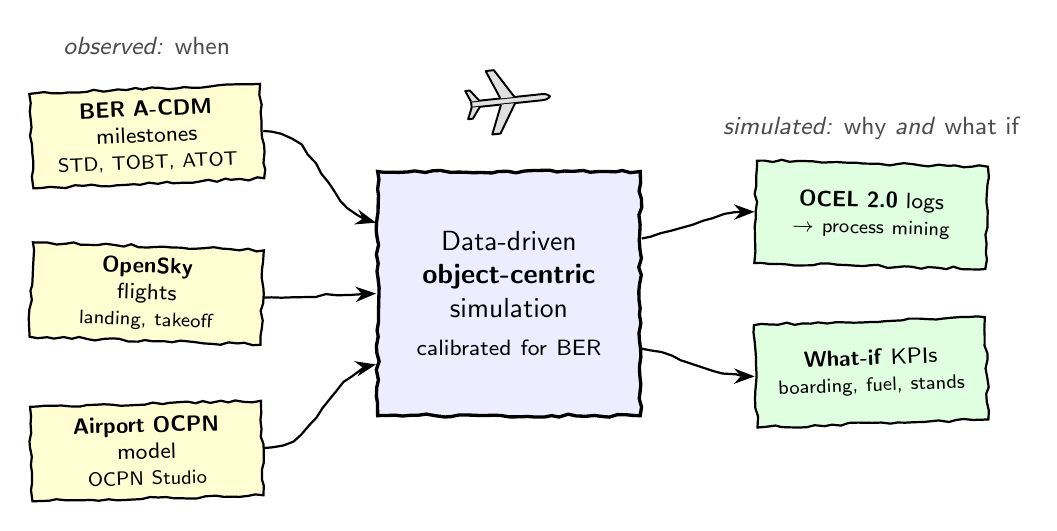
\begin{tikzpicture}[
  pen/.style={decorate, decoration={random steps, segment length=3pt, amplitude=0.55pt}},
  note/.style={draw, thick, pen, fill=yellow!18, align=center, font=\sffamily\footnotesize, text width=27mm, minimum height=12mm},
  core/.style={draw, very thick, pen, fill=blue!7, align=center, font=\sffamily, text width=31mm, minimum height=31mm},
  outbox/.style={draw, thick, pen, fill=green!12, align=center, font=\sffamily\footnotesize, text width=27mm, minimum height=13mm},
  harr/.style={thick, -{Stealth[length=2.6mm]}, decorate, decoration={random steps, segment length=4pt, amplitude=0.5pt, pre length=3pt, post length=4pt}},
  hand/.style={font=\sffamily\small\itshape, text=black!70, align=center}]
\pgfmathsetseed{11}
% inputs: what we can observe
\node[note, rotate=2.5]  (acdm)  at (0, 2.0) {\textbf{BER A-CDM}\\milestones\\{\scriptsize STD, TOBT, ATOT}};
\node[note, rotate=-2]   (osky)  at (0, 0)    {\textbf{OpenSky}\\flights\\{\scriptsize landing, takeoff}};
\node[note, rotate=1.5]  (model) at (0,-2.0) {\textbf{Airport OCPN}\\model\\{\scriptsize OCPN Studio}};
% the simulation
\node[core] (sim) at (4.6,0) {Data-driven\\\textbf{object-centric}\\simulation\\[2pt]{\footnotesize calibrated for BER}};
% outputs: what the simulation adds
\node[outbox, rotate=-1.5] (ocel) at (9.2, 1.0) {\textbf{OCEL 2.0} logs\\{\scriptsize $\to$ process mining}};
\node[outbox, rotate=2]    (kpi)  at (9.2,-1.0) {\textbf{What-if} KPIs\\{\scriptsize boarding, fuel, stands}};
% arrows
\draw[harr] (acdm.east)  to[out=0,  in=165] ([yshift=9mm]sim.west);
\draw[harr] (osky.east)  -- (sim.west);
\draw[harr] (model.east) to[out=0,  in=195] ([yshift=-9mm]sim.west);
\draw[harr] ([yshift=7mm]sim.east)  to[out=10,  in=180] (ocel.west);
\draw[harr] ([yshift=-7mm]sim.east) to[out=-10, in=180] (kpi.west);
% handwritten notes
\node[hand] at (0, 3.15) {observed: \emph{when}};
\node[hand] at (9.2, 2.1) {simulated: \emph{why} and \emph{what if}};
% a small aircraft sketch above the simulation
\begin{scope}[shift={(4.6,2.45)}, scale=0.3, rotate=6, line width=0.7pt]
  \draw[fill=black!12, line join=round] (-1.6,0.13) -- (1.2,0.13) .. controls (1.6,0.13) .. (1.75,0) .. controls (1.6,-0.13) .. (1.2,-0.13) -- (-1.6,-0.13) -- cycle;
  \draw[fill=black!12, line join=round] (0.25,0.13) -- (-0.5,1.35) -- (-0.85,1.35) -- (-0.35,0.13);
  \draw[fill=black!12, line join=round] (0.25,-0.13) -- (-0.5,-1.35) -- (-0.85,-1.35) -- (-0.35,-0.13);
  \draw[fill=black!12, line join=round] (-1.25,0.13) -- (-1.6,0.6) -- (-1.8,0.6) -- (-1.6,0.13);
  \draw[fill=black!12, line join=round] (-1.25,-0.13) -- (-1.6,-0.6) -- (-1.8,-0.6) -- (-1.6,-0.13);
\end{scope}
\end{tikzpicture}
\caption{Conceptual input--output view of the approach. Sparse operational milestones calibrate and evaluate an object-centric simulation, which produces OCEL~2.0 for process mining and key performance indicators (KPIs) for resource what-if analysis.}
\label{fig:inputoutput}
\end{figure}

\section{Motivation}
\label{sec:motivation}

The aircraft turnaround has been identified as one of the major contributors to airline delay, in particular through reactionary delay, that is, delay passed on from an earlier flight~\cite{evler2021recovery}. The turnaround is the point at which this transfer happens: if the inbound aircraft lands late and the scheduled ground time contains too little buffer, the outbound flight inherits the delay. Whether it does depends on how far the turnaround can be compressed, and this in turn depends on parallel activities and on the availability of shared resources. Delay propagation is therefore an object-centric phenomenon. It involves the aircraft, the turnaround, the stand and the resources that serve several aircraft in sequence.

Existing simulation studies represent these dependencies well, for example with timed Petri nets~\cite{sng2019petri,cui2024ttpn} or discrete-event models~\cite{tang2024covid,purohit2026intact}. However, they are usually calibrated with recorded activity durations, which are rarely shared outside an airline or ground handler. Studies that rely only on public data, on the other hand, can describe milestones but not the processes between them~\cite{schultz2021adsb}. A recent bachelor thesis reconstructs turnaround traces at Frankfurt Airport from in-block and off-block boundaries and exports them as OCEL~2.0~\cite{tkacenko2026}. It shows that agreement with the total turnaround duration does not guarantee agreement for the individual activities. Its durations are taken from the literature, candidate traces are selected by Monte Carlo rejection sampling, and it evaluates thirteen reference turnarounds.

This thesis takes the next step. Instead of assuming durations and filtering simulated traces to match observations, we first ask which properties of the turnaround the available milestones \emph{do} reveal, use them to calibrate carrier-specific service times, and simulate every observed day once instead of sampling many random candidates. Consider a short example. On 1 November 2026, Eurowings flight EWG43J was scheduled to leave BER only 27 minutes after its inbound aircraft was last observed on approach. The airline set the TOBT 30 minutes after the scheduled time. The A-CDM record alone cannot tell us which activity caused this. A calibrated object-centric simulation can show which resource the aircraft waited for, which branch finished last, and how the result would change with faster boarding or an additional fuel truck. This example is followed throughout Chapter~\ref{ch:methods}.

\section{Problem Statement}
\label{sec:problem}

Detailed event logs of aircraft turnarounds are not available at BER, as at most airports. What is available are two kinds of sparse observations. First, BER operates an A-CDM application, a live departure board for airport partners that lists the A-CDM milestones of every departing flight (scheduled, target and actual times, stand and runway). Second, the OpenSky Network provides surveillance-based flight observations from a community receiver network. Neither source records the start and end of ground services. At the same time, an existing object-centric Petri net of airport ground handling, published with OCPN Studio~\cite{ocpn_studio}, represents the relevant services and resources in detail, but its timing parameters are not derived from BER observations.

The problem addressed in this thesis is to connect these two worlds: to determine which turnaround properties can be measured from sparse milestones, to use them to calibrate and validate an object-centric simulation, and to use the resulting model to analyze waiting, delay propagation and resource allocation. The generated events must remain clearly separated from the observations, so that the simulation can support analysis without being mistaken for measured data.

\section{Research Questions}
\label{sec:rq}

Building on this problem, we define the following research questions (RQ):
\begin{description}
\item[RQ1:] To what extent can A-CDM departure milestones, linked to the arrival of the same aircraft, be used to calibrate the service times of an OCPN turnaround simulation, and how well does the calibrated model reproduce turnaround times on days not used for calibration?
\item[RQ2:] How do dependencies between aircraft, stands and shared ground-service resources contribute to waiting times and delay propagation at terminal and remote stands in an OCPN simulation?
\item[RQ3:] How can the calibrated simulation be used to evaluate resource-allocation strategies and identify configurations that reduce turnaround delays and resource contention?
\end{description}
Together, these questions lead from the data to the model (RQ1), from the model to an explanation of observed delay patterns (RQ2) and from the explanation to operational decisions (RQ3).

\section{Research Goals}
\label{sec:goals}

To answer the research questions systematically, we establish the following research goals:
\begin{enumerate}
\item Build an auditable BER dataset that links A-CDM departure milestones with OpenSky observations of the same aircraft, and enrich it with carrier class, aircraft type and observed weather.
\item Derive empirical turnaround properties, delay drivers and early-warning classifiers from these observations, and test them on held-out data.
\item Extend the airport ground-handling OCPN of OCPN Studio~\cite{ocpn_studio} with carrier-specific service times, observed weather, the BER night regulation and schedule-bound departures, and calibrate it against the observed targets.
\item Simulate all observed days, analyze the generated OCEL~2.0 logs with object-centric process mining, and evaluate process, capacity and allocation scenarios.
\end{enumerate}

\section{Contributions}
\label{sec:contrib}

Addressing these goals yields empirical findings, models and software artifacts. The main contributions are:
\begin{itemize}
\item A linked and enriched BER dataset: 1,322 A-CDM departure records cross-checked against OpenSky (97.7\% unique correspondence, median absolute difference eight seconds), 610 turnarounds linked to their inbound flight, and 10,212 in-scope turnarounds over 41 days with carrier class, aircraft type and hourly weather. A second dataset of 2,067 turnarounds from February to April 2026, recorded manually in previous work (the \emph{previous-work dataset}), is used for held-out evaluation.
\item Empirical turnaround properties (buffer-dependent delay transfer, target turnaround times by carrier class, runway contention, rotation carry-over), estimates of the drivers of departure delay, and an early-warning classifier that flags late departure targets at landing with an AUC of about 0.8.
\item A carrier-specific extension of the airport ground-handling OCPN with observed weather, the BER night regulation and schedule binding, calibrated against A-CDM targets with a 36--72\% reduction of the error on three held-out days.
\item An evaluation in which each scenario is simulated on all 41 observed days, an object-centric process-mining analysis of the generated logs (discovery, conformance, performance spectrum, friction analysis), and a paired evaluation of process, capacity and stand-allocation scenarios.
\end{itemize}
The process structure and resource logic of the airport model are taken from previous work~\cite{ocpn_studio}; this thesis contributes the BER adaptation, the calibration and the analyses.

\section{Thesis Structure}
\label{sec:structure}

The remainder of this thesis is organized as follows. Chapter~\ref{ch:prelim} introduces the formal foundations: OCEL~2.0, object-centric Petri nets, A-CDM milestones, object-centric discovery and conformance, and the statistical methods used. Chapter~\ref{ch:related} reviews related work. Chapter~\ref{ch:methods} presents the proposed pipeline, from data linkage to calibration targets, simulation and event-log export, followed by its implementation in Chapter~\ref{ch:implementation}. Chapter~\ref{ch:evaluation} evaluates the approach, and Chapter~\ref{ch:discussion} discusses the findings, their practical value and their limitations. Finally, Chapter~\ref{ch:conclusion} summarizes the contributions and outlines future work.

\cleardoublepage
\chapter{Foundations: Object-Centric Event Data, Petri Nets and A-CDM}
\label{ch:prelim}

This chapter introduces the concepts on which the rest of the thesis builds: the event data the simulation produces, the Petri nets that produce them, the milestones they are compared with, and the techniques used to analyze and compare them.

\section{Object-Centric Event Logs (OCEL 2.0)}
\label{sec:prelim-ocel}

Traditional event logs assign every event to exactly one case. In a turnaround, however, a single event such as \emph{start fueling} concerns an aircraft, a turnaround, a fuel truck and a stand at the same time. Forcing such data into one case notion leads to convergence and divergence problems~\cite{berti2023ocpmreview}. OCEL~2.0 avoids this by relating each event to any number of objects~\cite{koren2024ocel2}. We use the following simplified definition, which follows the OCEL~2.0 specification.

\begin{definition}[Universes]
Let $\mathcal{U}_{ev}$, $\mathcal{U}_{etype}$, $\mathcal{U}_{obj}$, $\mathcal{U}_{otype}$, $\mathcal{U}_{attr}$, $\mathcal{U}_{val}$, $\mathcal{U}_{qual}$ be pairwise disjoint universes of event identifiers, event types, object identifiers, object types, attribute names, attribute values and relationship qualifiers. $\mathcal{U}_{time}$ denotes the universe of timestamps.
\end{definition}

\begin{definition}[Object-centric event log]
\label{def:ocel}
An object-centric event log is a tuple
\[
L=(E,O,\mathit{evtype},\mathit{time},\mathit{objtype},\mathit{eaval},\mathit{oaval},E2O,O2O)
\]
where
\begin{itemize}
\item $E\subseteq\mathcal{U}_{ev}$ and $O\subseteq\mathcal{U}_{obj}$ are finite sets of events and objects,
\item $\mathit{evtype}:E\to\mathcal{U}_{etype}$ and $\mathit{objtype}:O\to\mathcal{U}_{otype}$ assign types,
\item $\mathit{time}:E\to\mathcal{U}_{time}$ assigns a timestamp to each event,
\item $\mathit{eaval}:E\times\mathcal{U}_{attr}\not\to\mathcal{U}_{val}$ assigns event attribute values,
\item $\mathit{oaval}:O\times\mathcal{U}_{attr}\times\mathcal{U}_{time}\not\to\mathcal{U}_{val}$ assigns object attribute values that may change over time,
\item $E2O\subseteq E\times\mathcal{U}_{qual}\times O$ is the set of qualified event-to-object relations, and
\item $O2O\subseteq O\times\mathcal{U}_{qual}\times O$ is the set of qualified object-to-object relations.
\end{itemize}
\end{definition}

For example, the event \emph{start fueling} of a turnaround $ta$ can be related to $ta$ with the qualifier \texttt{turnaround}, to the aircraft with \texttt{aircraft} and to a fuel tanker with \texttt{fueller}. An O2O relation records the stand at which the turnaround is \texttt{parked at}. Since resources are objects of their own, their whole lifecycle across many turnarounds becomes visible in the log.

\section{Timed Colored Petri Nets and Object-Centric Models}
\label{sec:prelim-cpn}

We model the operational behavior with timed colored Petri nets (CPNs)~\cite{jensen2009cpn}. Tokens carry data values (\emph{colors}) and timestamps, which makes it possible to represent individual aircraft and resources as distinguishable tokens.

\begin{definition}[Timed colored Petri net]
\label{def:cpn}
A timed CPN is a tuple $N=(P,T,F,\Sigma,V,C,G,E,I)$, where $P$ and $T$ are finite disjoint sets of places and transitions, $F\subseteq(P\times T)\cup(T\times P)$ is a set of arcs, $\Sigma$ is a finite set of (possibly timed) color sets, $V$ is a set of typed variables, $C:P\to\Sigma$ assigns a color set to every place, $G$ assigns a Boolean guard expression to every transition, $E$ assigns an arc expression to every arc, and $I$ assigns an initial timed multiset of tokens to every place.
\end{definition}

A token $c@\tau$ has value $c$ and becomes available at time $\tau$. A transition is enabled when every input place contains tokens that satisfy the arc expressions and the guard, and all of these tokens are available. When it fires, it consumes these tokens and produces new tokens whose timestamps may be increased by a delay. Stochastic delays are obtained by sampling from probability distributions in the arc or transition expressions.

\paragraph{Object-centric interpretation.}
Object-centric Petri nets associate places with object types and allow transitions to consume and produce several objects of different types at once~\cite{vanderaalst2020ocpn}. The model used in this thesis is built in OCPN Studio~\cite{ocpn_studio} and executed by the CPNsim runtime~\cite{cpnsim}. It follows this interpretation: each color set of record type corresponds to an object type, such as \texttt{Aircraft}, \texttt{Turnaround}, \texttt{Stand} or \texttt{Fueller}, and each token of such a color set represents one object. Color sets of simple types, such as integers or strings, carry auxiliary values and do not define object types. A transition firing therefore corresponds to an event that relates all objects it consumes or produces. This correspondence is the basis of the OCEL export in Section~\ref{sec:method-ocel}.

\paragraph{Synchronization.}
A turnaround splits into parallel handling branches that must all be completed before the aircraft can leave. In a Petri net, this is a join transition that requires one token from every branch. We call the branch whose token becomes available last the \emph{last-ready branch} of a turnaround. It determines when the join can fire, and it is the object-centric counterpart of the critical path in a project schedule.

\section{A-CDM Milestones}
\label{sec:prelim-acdm}

A-CDM defines a sequence of milestones that partners share about each flight~\cite{eurocontrol_acdm}. For a departure $d$ we write:
\begin{itemize}
\item $\mathrm{STD}_d$, the scheduled time of departure from the timetable,
\item $\mathrm{EOBT}_d$, the estimated off-block time from the flight plan,
\item $\mathrm{TOBT}_d$, the target off-block time, that is, the time at which the aircraft operator or ground handler expects the aircraft to be ready, with doors closed and boarding bridge removed,
\item $\mathrm{TSAT}_d$, the target start-up approval time issued by the pre-departure sequencer, and
\item $\mathrm{ATOT}_d$, the actual takeoff time.
\end{itemize}
TOBT and TSAT are \emph{targets}: they are set and updated during the turnaround, and the published value is typically the last one. ATOT is an \emph{actual} time. In-block (AIBT) and off-block (AOBT) times are part of the full milestone concept but are not published by the BER application used in this thesis.

\begin{definition}[Turnaround observation]
\label{def:taobs}
A turnaround observation is a pair $(a,d)$ of an inbound flight $a$ and the next departure $d$ of the same aircraft from the same airport. Let $t_a^{\mathrm{land}}$ be an observed landing time of $a$. We define the \emph{scheduled buffer}
\[
B_{(a,d)}=\mathrm{STD}_d-t_a^{\mathrm{land}}
\]
and the \emph{target turnaround time} $\mathrm{TTA}_{(a,d)}=\mathrm{TOBT}_d-t_a^{\mathrm{land}}$. The \emph{target shift} $\Delta^{\mathrm{TOBT}}_d=\mathrm{TOBT}_d-\mathrm{STD}_d$ measures by how much the operator expects to be late.
\end{definition}

A small or negative buffer means that the inbound aircraft has little time to be turned around before its scheduled departure. If the target shift grows as the buffer shrinks, inbound delay is being transferred to the outbound flight. Chapter~\ref{ch:methods} uses this relation as a calibration target.

\section{Object-Centric Process Discovery and Conformance}
\label{sec:prelim-pm}

Process discovery constructs a process model from an event log, and conformance checking measures how well a log and a model agree~\cite{vanderaalst2016pm}. For object-centric logs, two families of models are used in this thesis.

\paragraph{Object-centric directly-follows graph (OC-DFG).}
For every object type $ot$, the events related to each object of that type are ordered by time. An edge $(a,b)$ of type $ot$ exists if some object of type $ot$ is related to an event of activity $a$ that is directly followed by an event of activity $b$. Each edge is annotated with its frequency or with the time between the two events. Because every object type contributes its own edges, the OC-DFG shows the lifecycle of aircraft, turnarounds and resources in one picture~\cite{vanderaalst2020ocpn,berti2023ocpmreview}.

\paragraph{Object-centric Petri net (OCPN).}
An OCPN is discovered by flattening the log per object type, discovering a Petri net for each type with the inductive miner and merging the nets at shared activities~\cite{vanderaalst2020ocpn}.

\paragraph{Flattening and conformance.}
\emph{Flattening} a log on object type $ot$ produces a traditional event log in which each object of type $ot$ is a case. Given a flattened log and a Petri net, token-based replay measures \emph{fitness} (the share of observed behavior the model can replay) and \emph{precision} (how little behavior the model allows beyond what is observed)~\cite{rozinat2008conformance}. Both lie in $[0,1]$.

\section{Trace-Driven Simulation and Statistical Comparison}
\label{sec:prelim-stats}

The simulation in this thesis is \emph{trace-driven}. A conventional simulation generates arrivals from a random process. Here, the input of each simulated day is instead the list of aircraft that were actually observed arriving at BER on that day, each with its landing time, airline and aircraft type. We call this list the \emph{observed arrival demand} of the day. Every scenario is executed once per day on the same arrival demand and the same observed weather, so that two scenarios differ only in the change that defines them.

\begin{definition}[Paired daily comparison]
Let $m_{s,d}$ be the mean of a metric over all turnarounds of day $d$ in scenario $s$. The effect of scenario $s$ relative to a reference $s_0$ is the mean paired difference $\bar\Delta_s=\frac{1}{D}\sum_{d=1}^{D}(m_{s,d}-m_{s_0,d})$ over $D$ days. Its 95\% confidence interval is $\bar\Delta_s\pm t_{0.975,D-1}\cdot \mathit{sd}/\sqrt{D}$, where $\mathit{sd}$ is the standard deviation of the $D$ daily differences and $t_{0.975,D-1}$ the quantile of Student's $t$-distribution with $D-1$ degrees of freedom~\cite{law2015simulation}.
\end{definition}

Using the operational day as the statistical unit accounts for the dependence between turnarounds that share resources within a day~\cite{law2015simulation}. Pairing by day removes the variation between days in demand and weather, so that a difference reflects the scenario. Monte Carlo replication, that is, repeating the same day many times with new random numbers, is used only as a comparison to quantify the run-to-run variability of the stochastic model. Two sets of replications are compared with a Welch interval, which does not assume equal variances~\cite{welch1947}.

For observed data we use rank-based and resampling methods, because delays are skewed and contain outliers. The Spearman rank correlation $\rho$ measures monotone association. Confidence intervals are obtained by the nonparametric bootstrap: observations, or whole days where observations within a day are dependent, are resampled with replacement, the statistic is recomputed, and the 2.5th and 97.5th percentiles form a 95\% interval~\cite{efron1993bootstrap}. Classifiers for early delay detection are evaluated by the area under the ROC curve (AUC), which equals the probability that a randomly chosen delayed case receives a higher score than a randomly chosen punctual one.

\section{Summary}

This chapter formalized object-centric event logs and the timed colored Petri nets that underlie the simulation model. It introduced the A-CDM milestones and the buffer and target-shift quantities that connect them to the turnaround, the object-centric discovery and conformance techniques used to analyze the generated logs, and the paired daily comparison and resampling statistics used in the evaluation. The next chapter reviews how these concepts have been used in earlier work on aircraft turnarounds.

\cleardoublepage
\chapter{Related Work: Turnaround Models, Milestone Data and Process Mining}
\label{ch:related}

This chapter places the proposed approach in the context of existing research on turnaround modeling, operational milestone data and process mining in aviation.

\section{Modeling and Simulating Aircraft Turnarounds}

Schultz et al.\ describe the turnaround as a set of stochastic processes that must synchronize before departure, and show how disturbances on the critical path affect later operations~\cite{schultz2012dynamic}. They provide reference distributions for narrowbody cleaning, fueling and boarding, which we use as service-time inputs. Schultz later presents a calibrated stochastic boarding model and shows that reliable boarding is a key to fast turnarounds~\cite{schultz2018boarding}; a related study discusses turnaround requirements after the pandemic~\cite{schultz2020postpandemic}.

Petri nets have been used repeatedly to represent the synchronization constraints of the turnaround. Liu and Qin model ground operations as a timed Petri net and identify the critical routing by simulation~\cite{liu2006timedpetri}. Sng and Hansman construct Petri nets for narrowbody and widebody turnarounds, calibrate them with empirical data from Singapore Changi Airport and evaluate procedural modifications with Monte Carlo simulation and critical-path analysis~\cite{sng2019petri}. Cui et al.\ combine a time transition Petri net with Bayesian updating to predict turnaround time from historical activity data~\cite{cui2024ttpn}. At a finer scale, P{\l}anda and Skorupski model boarding as a hierarchical timed colored Petri net and show that disturbances can change the ranking of boarding strategies~\cite{planda2025boarding}. Discrete-event simulation has also been used to compare turnaround scenarios, for example pandemic-related process changes~\cite{tang2024covid} and new turnaround technologies~\cite{purohit2026intact}.

Activity durations differ between airline business models. Oreschko et al.\ show significant turnaround process variations due to airport characteristics~\cite{oreschko2010variations}, Asadi studies robust turnaround management under uncertainty and provides stochastic duration models for ground operations~\cite{asadi2024robust}, and Luo et al.\ record low-cost turnaround activities at Amsterdam Schiphol for an agent-based digital twin and use simulated ground times to train machine-learning predictors~\cite{luo2024digitaltwin,luo2021agent}. Tkacenko combines these sources into carrier-specific distributions~\cite{tkacenko2026}, which we adopt and calibrate for BER.

These studies demonstrate that Petri nets and simulation capture concurrency, synchronization and stochastic durations well. Their calibration, however, relies on recorded durations of individual activities, which are rarely available outside an airline or ground handler. Our approach keeps the same structural idea, but calibrates against properties that can be derived from publicly shared milestones.

\section{Resource Allocation and Delay Propagation}

Ground-handling resources are commonly studied as a scheduling or allocation problem. Padr\'on and Guimarans schedule interrelated ground-handling operations across several turnarounds~\cite{padron2019scheduling}, and C\'ile\v{c}ek et al.\ formulate staffing with substitutable personnel as a mathematical program~\cite{cilecek2024staffing}. Chen et al.\ combine task allocation and path planning for automated ground support equipment in a multi-agent system~\cite{chen2023multiagent}. Simulation-based studies are closest to our experimental design: Saha and Tomasella compare static and dynamic operational policies for allocating turnaround teams~\cite{saha2021policies}, and Saggar and Tomasella examine the planning and real-time allocation of ground support equipment~\cite{saggar2021gse}. El Asri et al.\ provide an overview of the field~\cite{elasri2018review}.

Delays that arise during a turnaround can propagate to later flights. Evler et al.\ integrate turnaround decisions into aircraft recovery to mitigate this propagation in airline networks~\cite{evler2021recovery}. Rodr\'iguez-Sanz et al.\ link inbound and outbound flights through A-CDM milestones in a Bayesian network built from about 34{,}000 turnarounds at Madrid-Barajas~\cite{rodriguezsanz2018uncertainty}. Purohit shows on 2.5 million US turnarounds that the availability of inbound status information matters more than its precision for predicting departure delay~\cite{purohit2026availability}. These works motivate our empirical properties P1 and P4, which measure delay transfer through the turnaround and along aircraft rotations.

\section{Operational Milestones: A-CDM and Surveillance Data}

EUROCONTROL describes A-CDM as an approach for sharing operational information among airport operators, aircraft operators, ground handlers, air traffic control and the Network Manager~\cite{eurocontrol_acdm}. Several studies use its milestones directly. Z\'u\~niga and Boosten derive capacity indicators from the milestone approach at Amsterdam Schiphol~\cite{zuniga2020cdm}, Li et al.\ evaluate multi-flight ground-handling performance from shared milestone information~\cite{li2022multiflight}, and Parente et al.\ describe the variation of TOBT and TSAT at S\~ao Paulo Guarulhos~\cite{parente2024guarulhos}. The TOBT itself is updated during the turnaround: Verkerk reports that many updates occur in the final minutes before off-block~\cite{verkerk2018tobt}, and Volt et al.\ show that TOBT predictions improve as ground-handling milestones become available~\cite{volt2026tobt}.

Surveillance data offer a complementary source. Schultz et al.\ derive operational milestones from ADS-B messages to support airports without a full A-CDM implementation~\cite{schultz2019acdmlite,schultz2021adsb}. The OpenSky Network provides such observations through a public API~\cite{opensky_rest}. We combine both sources: OpenSky identifies the physical aircraft and its arrival, and A-CDM provides the operator's target and the actual takeoff.

\section{Process Mining in Aviation}

Process mining has been applied to aviation operations mainly with case-centric event logs. Gunnarsson et al.\ apply predictive process monitoring to operational logistics in aviation~\cite{gunnarsson2019ppm}. Predictive process monitoring forecasts the remaining behavior of running cases, and object-centric logs have been shown to improve such predictions~\cite{fioretto2025ppm}. Our early-warning classifier follows this idea with the milestones available at landing. Rott et al.\ analyze the turnaround process at Munich Airport with process mining on A-CDM milestone data, and report that manually recorded timestamps can produce implausible sequences~\cite{rott2023processmining}. In both cases, the flight or turnaround is the case, and the resources shared between turnarounds are not represented as objects of their own.

Tkacenko addresses the missing data with simulation~\cite{tkacenko2026}. The study models narrowbody turnarounds at Frankfurt Airport as a timed CPN in \texttt{cpn-py}, generates candidate traces by Monte Carlo simulation and exports them as OCEL~2.0. Candidates are accepted if their simulated off-block time falls within a window around the observed one, and the accepted traces are compared with 13 reference turnarounds recorded by computer vision. The study shows that agreement with the total turnaround duration does not imply agreement for the individual activities, and demonstrates a what-if analysis with an additional baggage loader.

\section{Object-Centric Process Mining}

Object-centric process mining relaxes the single-case assumption, so that an event can refer to several objects of different types~\cite{berti2023ocpmreview}. OCEL~2.0 adds explicit object-to-object relations, relationship qualifiers and evolving object attributes~\cite{koren2024ocel2,ocel2}, and object-centric Petri nets provide a matching process model~\cite{vanderaalst2020ocpn}. A recent community manifesto aligns terminology and research challenges for object-centric process management~\cite{seidel2026manifesto}. Tools such as Promenade support the exploration of object-centric logs~\cite{promenade}. Berti et al.\ note that adoption in real-world analyses is still limited~\cite{berti2023ocpmreview}.

\section{Positioning of this Thesis}

Table~\ref{tab:positioning} compares this thesis with the three studies that are closest to it: a Petri-net simulation calibrated with recorded activity data~\cite{sng2019petri}, a process-mining analysis of A-CDM milestones~\cite{rott2023processmining}, and a simulation that generates OCEL~2.0 logs for turnarounds~\cite{tkacenko2026}. The rows of the table follow the steps that every data-driven turnaround study has to take, and that structure the method of this thesis (Chapter~\ref{ch:methods}): the airport studied, the data used, the formalism of the model, the type of event log, how the model is calibrated, how it is validated, and which what-if questions it answers. The distinguishing features of this thesis are the combination of an object-centric simulation with empirical properties derived from public milestones of a real airport, a held-out evaluation, and what-if experiments on 41 observed days.

\begin{table}[htbp]\centering\footnotesize
\begin{tabular}{p{2.1cm}p{2.2cm}p{2.2cm}p{2.4cm}p{2.7cm}}\hline
& Sng \& Hansman~\cite{sng2019petri} & Rott et al.~\cite{rott2023processmining} & Tkacenko~\cite{tkacenko2026} & This thesis\\\hline
Airport & Changi & Munich & Frankfurt & Berlin Brandenburg\\\hline
Data & Activity records & A-CDM milestones & IBT/OBT, 13 CV traces & A-CDM, OpenSky, weather, previous-work dataset\\\hline
Formalism & Petri net & Process mining & Timed CPN & Object-centric Petri net\\\hline
Event log & -- & Case-centric & OCEL~2.0 & OCEL~2.0\\\hline
Calibration & Activity durations & -- & Literature, rejection sampling & Carrier-specific, grid calibration on A-CDM targets\\\hline
Validation & Empirical calibration data & -- & 13 reference turnarounds & Held-out days, 41 days, second season\\\hline
What-if & Procedures & -- & 1 vs.\ 2 loaders & Boarding, fuel, buses, loaders, stand allocation (41 days)\\\hline
\end{tabular}
\caption{Positioning of this thesis relative to the closest related studies. The rows are the steps of a data-driven turnaround study, from the data source to the what-if analysis. IBT/OBT: in-block and off-block times; CV: computer vision.}
\label{tab:positioning}
\end{table}

\section{Summary}

The literature establishes Petri nets and simulation as suitable means to represent turnaround dependencies, and shows the value of A-CDM milestones and process mining for analyzing recorded operations. It also shows that detailed activity data, needed for calibration, are rarely available. Building on these foundations, this thesis connects an object-centric turnaround simulation with empirical properties that can be derived from public milestones. The next chapter describes how.

\cleardoublepage
\chapter{From Sparse Milestones to a Calibrated Object-Centric Simulation}
\label{ch:methods}

This chapter introduces the proposed approach for a data-driven object-centric turnaround simulation. The core challenge is that the available observations describe the boundaries of the turnaround (the arrival of the aircraft and the departure milestones), but not the ground services between them. We therefore do not try to reconstruct every service from these boundaries. Instead, we derive turnaround properties that the boundaries \emph{do} reveal, use them to calibrate a detailed simulation model with carrier-specific service times, and analyze the generated object-centric event logs with process mining. The approach is a five-step pipeline, shown in Figure~\ref{fig:pipeline}:

\begin{enumerate}
\item \textbf{Data acquisition, linkage and enrichment (Section~\ref{sec:method-data}):} We collect departure milestones from the BER A-CDM application and surveillance observations from the OpenSky Network, link each departure to the inbound flight of the same aircraft, and enrich every turnaround with airline, carrier class, aircraft type and observed weather.
\item \textbf{Empirical turnaround properties and early warning (Section~\ref{sec:method-targets}):} From the linked observations we derive properties that characterize how BER turnarounds absorb or transfer delay, estimate the drivers of delay, and build classifiers that flag a late departure when the inbound aircraft lands.
\item \textbf{Object-centric simulation (Section~\ref{sec:method-model}):} We adapt the extended airport OCPN to BER: observed arrivals, carrier-specific service times, observed weather, the BER night regulation and schedule-bound departures.
\item \textbf{Calibration and experiments (Section~\ref{sec:method-calibration}):} Two carrier-specific multipliers are calibrated against observed A-CDM targets on two days and validated on a third; the calibrated model is then run on all 41 days for timing and resource scenarios.
\item \textbf{OCEL~2.0 export and process mining (Section~\ref{sec:method-ocel}):} Simulated days are exported as object-centric event logs, analyzed with PM4Py (discovery and conformance) and explored in Promenade.
\end{enumerate}

\begin{figure}[htbp]
\centering
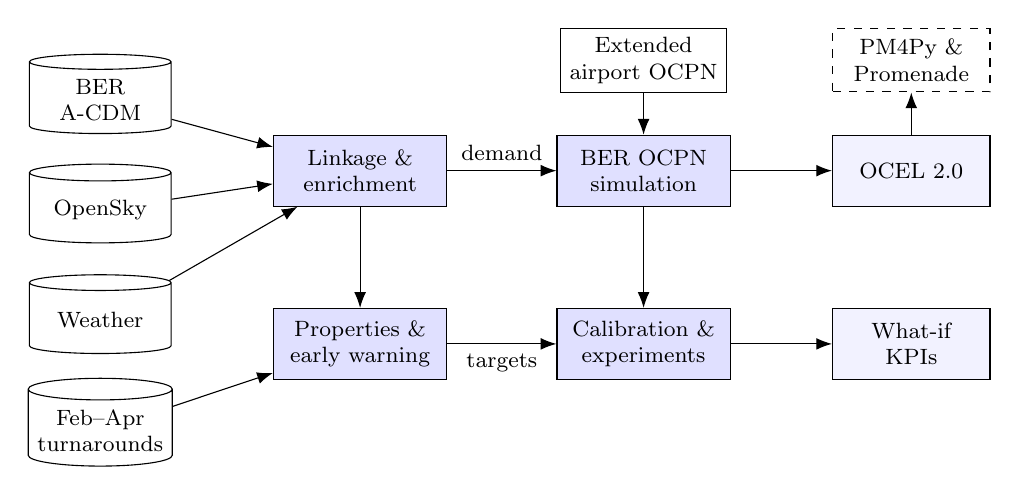
\begin{tikzpicture}[
  font=\footnotesize,
  inp/.style={draw, rectangle, minimum width=20mm, minimum height=8mm, align=center},
  db/.style={draw, cylinder, shape border rotate=90, aspect=0.15, minimum width=18mm, minimum height=10mm, align=center},
  dev/.style={draw, rectangle, fill=blue!12, minimum width=22mm, minimum height=9mm, align=center},
  art/.style={draw, rectangle, fill=blue!5, minimum width=20mm, minimum height=9mm, align=center},
  tgt/.style={draw, dashed, rectangle, minimum width=20mm, minimum height=8mm, align=center},
  arr/.style={-{Latex[length=2mm]}}]
\node[db] (acdm) at (0,2.1) {BER\\A-CDM};
\node[db] (osky) at (0,0.7) {OpenSky};
\node[db] (wx) at (0,-0.7) {Weather};
\node[db] (man) at (0,-2.1) {Feb--Apr\\turnarounds};
\node[dev] (link) at (3.3,1.2) {Linkage \&\\enrichment};
\node[dev] (props) at (3.3,-1.0) {Properties \&\\early warning};
\node[inp] (base) at (6.9,2.6) {Extended\\airport OCPN};
\node[dev] (sim) at (6.9,1.2) {BER OCPN\\simulation};
\node[dev] (exp) at (6.9,-1.0) {Calibration \&\\experiments};
\node[art] (ocel) at (10.3,1.2) {OCEL 2.0};
\node[tgt] (pm) at (10.3,2.6) {PM4Py \&\\Promenade};
\node[art] (kpi) at (10.3,-1.0) {What-if\\KPIs};
\draw[arr] (acdm) -- (link);
\draw[arr] (osky) -- (link);
\draw[arr] (wx) -- (link);
\draw[arr] (link) -- (props);
\draw[arr] (man) -- (props);
\draw[arr] (link) -- node[above]{demand} (sim);
\draw[arr] (base) -- (sim);
\draw[arr] (sim) -- (ocel);
\draw[arr] (ocel) -- (pm);
\draw[arr] (sim) -- (exp);
\draw[arr] (props) -- node[below]{targets} (exp);
\draw[arr] (exp) -- (kpi);
\end{tikzpicture}
\caption{Data and execution flow of the proposed pipeline. Feb--Apr turnarounds: the manually recorded turnarounds of February to April 2026 (Section~\ref{sec:method-febapr}). Observations are linked, enriched and summarized into empirical properties; observed arrivals drive the simulation; the properties calibrate and evaluate its output, which is exported as OCEL~2.0 for process mining and used for what-if analysis.}
\label{fig:pipeline}
\end{figure}

\paragraph{Running example.}
To make the steps concrete, we follow one turnaround throughout this chapter. On 1 November 2026, a Eurowings Airbus A320neo (registration D-AENB) arrived at BER from London Heathrow and departed as flight EWG43J to Zurich. It was parked at stand B04. Its inbound flight was last observed by OpenSky at 16:42:37~UTC. The following sections show how this aircraft is linked across sources, which properties it contributes to and how it is represented in the simulation and in the event log.

\section{Data Acquisition, Linkage and Enrichment}
\label{sec:method-data}

\subsection{BER A-CDM Departure Milestones}
The BER A-CDM application is a live departure board: it shows the current state of each departing flight, and its target times change whenever the airline or the ground handler updates them. We do not record these updates. Instead, a collector retrieves the board once per day, shortly after midnight, for the calendar day that has just ended. At that point every flight of the day has departed, and the board contains the final value of each milestone. The collector stores the raw responses and writes a table filtered to the requested date (Chapter~\ref{ch:implementation}). The collection used in this thesis covers five operational days (1, 5, 8, 15 and 16~November~2026) with 1,322 departure records. Each record contains the callsign, flight number, aircraft registration and type, airline, destination, stand and gate, runway, and the milestones STD, EOBT, TOBT, TSAT and ATOT (Section~\ref{sec:prelim-acdm}). The board does not contain arrival, in-block or off-block milestones, nor any ground-service timestamps.

Records are retained in a master table even when they are canceled or incomplete. A record is \emph{eligible} for departure analysis when it has a valid identifier, date and an actual takeoff, which holds for 1,286 records. A complete TOBT/TSAT/ATOT triple exists for 1,283 of them. The application publishes timestamps without a timezone. We test two interpretations, UTC and Europe/Berlin, in the cross-check below and adopt the one that the independent data support.

For the running example, the A-CDM record of EWG43J gives $\mathrm{STD}=17{:}10$, $\mathrm{TOBT}=\mathrm{TSAT}=17{:}40$ and $\mathrm{ATOT}=17{:}49{:}36$, with stand B04 and runway 06L.

\subsection{OpenSky Surveillance Observations}
The OpenSky Network provides, for each flight observed by its receivers, the aircraft's ICAO24 transponder address, the callsign, the first and last observation time and the estimated departure and arrival airports~\cite{opensky_rest}. For an arrival at BER, the last observation $t^{\mathrm{last}}_a$ occurs shortly before touchdown or during the landing roll, depending on receiver coverage. We therefore use it as a \emph{landing proxy}. For a departure, the first observation $t^{\mathrm{first}}_d$ occurs shortly after takeoff. The prepared movement table contains 11,316 BER arrivals and 11,319 departures between 30~September and 9~November~2026.

\subsection{Aircraft Pairing and A-CDM Linkage}
Since the ICAO24 address identifies a physical aircraft, consecutive movements of the same address form candidate turnarounds.

\begin{definition}[Candidate turnaround]
Let $M_x$ be the time-ordered BER movements of aircraft $x$. Every arrival $a\in M_x$ that is directly followed by a departure $d\in M_x$ forms a candidate turnaround $(a,d)$ with ground interval proxy $G_{(a,d)}=t^{\mathrm{first}}_d-t^{\mathrm{last}}_a$.
\end{definition}

Candidates are screened for plausibility (for example, implausible airport assignments or competing airport candidates), which yields 10,940 core candidate turnarounds over 41 arrival days. Of these, 8,951 have a ground interval between 15~minutes and six hours, and 1,989 between six and 24~hours. The long intervals usually include overnight parking or timetable gaps rather than continuous handling.

An A-CDM departure is linked to an OpenSky departure if the normalized callsigns agree and the OpenSky first observation lies within 30~minutes of the interpreted ATOT. A link is retained only if it is unique in both directions. Through the OpenSky departure, the A-CDM record inherits the inbound flight of the same aircraft. This produces the linked dataset used for the empirical properties: 610 turnarounds with a complete A-CDM triple, a ground interval below six hours and an inbound landing proxy, on the three days covered by both sources (1, 5 and 8~November).

In the running example, the OpenSky departure of ICAO24 \texttt{3c55c2} was first observed 2~seconds before the A-CDM ATOT. The same aircraft's previous flight, from London Heathrow, was last observed at 16:42:37. The candidate turnaround therefore has a ground interval proxy of $66.95$~minutes and a scheduled buffer of $B=17{:}10-16{:}42{:}37=27.4$~minutes.

\subsection{Enrichment: Airline, Carrier Class, Aircraft Type and Weather}
Every candidate turnaround is enriched with four attributes.
\begin{itemize}
\item \textbf{Airline.} The ICAO designator is taken from the outbound callsign (available for 99\% of turnarounds).
\item \textbf{Carrier class.} Airlines are classified as \emph{low-cost}, \emph{full-service} or \emph{leisure} (charter and holiday carriers). Where an airline appears in the February--April collection (Section~\ref{sec:method-febapr}), the class recorded there is used; the remaining airlines are classified by business model (Appendix~\ref{app:details}). Military flights, business aviation and cargo operators are excluded from the scope.
\item \textbf{Aircraft type.} The type is taken from the linked A-CDM record or, otherwise, from the OpenSky aircraft database (77\% coverage); unknown types fall back to an A320 configuration.
\item \textbf{Weather.} Hourly observed weather at BER (temperature, precipitation, snowfall, wind speed and gusts, cloud cover) is retrieved from the Open-Meteo historical archive~\cite{openmeteo}, which is based on the ERA5 reanalysis~\cite{hersbach2020era5}, and joined to each turnaround by the hour of arrival.
\end{itemize}
After exclusion, 10,212 turnarounds are in scope: 4,963 low-cost, 3,993 full-service, 928 leisure and 328 other commercial turnarounds.

\subsection{Second Dataset: February to April 2026}
\label{sec:method-febapr}
Before the A-CDM collector was available, turnarounds were recorded manually from the BER A-CDM application on twenty days: 21~February to 4~March and 17 to 24~April~2026. Each of the 2,070 records pairs an inbound and an outbound flight number of the same airline at the same gate. It contains the scheduled and actual landing time of the inbound flight, the scheduled and actual departure time of the outbound flight, the gate and an airline class (full-service or low-cost). Three records with an actual ground time below 15~minutes or a delay above 300~minutes are excluded as transcription errors, which leaves 2,067. In contrast to the linked November data, the inbound and outbound flights are paired by flight number rather than by aircraft identity.

\section{Empirical Turnaround Properties and Early Warning}
\label{sec:method-targets}

The observations do not show when cleaning or fueling took place. They do show how the turnaround as a whole reacts to time pressure. We derive four properties that the simulation should reproduce if its services, resources and dependencies are represented adequately.

\paragraph{P1: Buffer-dependent delay transfer (RQ1, RQ2).}
For each linked turnaround we relate the target shift $\Delta^{\mathrm{TOBT}}$ to the scheduled buffer $B$ (Definition~\ref{def:taobs}). The share of turnarounds with $\Delta^{\mathrm{TOBT}}>5$~minutes, as a function of $B$, is the empirical delay-transfer curve.

\paragraph{P2: Target turnaround time (RQ1).}
The target turnaround time $\mathrm{TTA}=\mathrm{TOBT}-t^{\mathrm{last}}_a$ measures how long the operator expects to need from landing until the aircraft is ready, including taxi-in. Its quantiles by carrier class are the main calibration target: the simulated time from arrival to \emph{Aircraft Ready} should have the same distribution. Under time pressure ($B<45$~minutes), its lower percentiles estimate the minimum feasible turnaround.

\paragraph{P3: Runway-bank contention (RQ2).}
For every departure we count the other departures whose TSAT lies within $\pm15$~minutes and relate this load to $\mathrm{ATOT}-\mathrm{TSAT}$.

\paragraph{P4: Delay carry-over along rotations (RQ2).}
When the same aircraft departs BER twice on one day, we relate the departure delay $\mathrm{ATOT}-\mathrm{STD}$ of the first departure to that of the second.

\paragraph{Delay drivers.}
On the February--April data, the outbound delay is related to the inbound delay, the carrier class, the time of day and the weather at landing (precipitation $\ge0.1$~mm/h, gusts $\ge40$~km/h, temperature $\le1\,^{\circ}$C), both as a linear model of the delay in minutes and as a logistic model of a delay above 15~minutes. Turnarounds of the same day are not independent observations: weather and traffic change during a day, but turnarounds close in time experience similar conditions, and a disruption affects many turnarounds of the same day. Confidence intervals are therefore obtained by resampling whole days rather than individual turnarounds, which keeps any dependence within a day intact.

\paragraph{Held-out delay-transfer model.}
To test P1 on independent data, we fit a reactionary-delay model on the February--March records and evaluate it on the April records. For a turnaround $i$ with inbound delay $\delta^{\mathrm{in}}_i$, scheduled ground time $S_i$ and an unknown minimum turnaround time $\mathrm{MTT}$, only the part of the inbound delay that exceeds the slack $S_i-\mathrm{MTT}$ should be transferred:
\begin{equation}
\delta^{\mathrm{out}}_i=\beta_0+\beta_1\max\bigl(0,\;\delta^{\mathrm{in}}_i-(S_i-\mathrm{MTT})\bigr)+\varepsilon_i.
\label{eq:transfer}
\end{equation}
MTT is estimated per airline class by a grid search, and the model is compared on the test period with full transfer and with a constant prediction.

\paragraph{Early warning.}
To detect delays early, we train classifiers that use only information available when the inbound aircraft lands: the scheduled buffer, carrier class, aircraft size, hour, the number of arrivals within $\pm60$~minutes and the weather. On the linked November data, the target is a late TOBT ($\Delta^{\mathrm{TOBT}}>5$~minutes) and the evaluation is leave-one-day-out; on the February--April data, the target is an outbound delay above 15~minutes, trained on February--March and tested on April. We compare logistic regression with gradient-boosted trees~\cite{pedregosa2011sklearn} and report the AUC and the precision when as many turnarounds are flagged as are actually late.

\paragraph{Disruption screening.}
To detect operational disruptions such as strikes, holiday peaks or weather events, daily indicators of the 10,940 OpenSky turnarounds (number of turnarounds, median ground time of short stays) are compared with a baseline for the same weekday and flight-schedule season. Days whose robust $z$-score exceeds 3 are flagged and checked against observed weather and public information.

For the running example, $B=27.4$~minutes and $\Delta^{\mathrm{TOBT}}=+30$~minutes, so the turnaround falls into the lowest buffer class of P1. Its target turnaround time is $17{:}40-16{:}42{:}37=57.4$~minutes.

\section{Object-Centric Simulation Model}
\label{sec:method-model}

\subsection{Baseline Model}
The simulation is based on the \emph{Airport Ground Handling (Extended)} model, which is published as an example model of OCPN Studio~\cite{ocpn_studio}. It represents a medium-sized European airport in six hierarchical nets: \emph{Airport}, \emph{Flight Schedule}, \emph{Approach, Landing \& Taxi In}, \emph{Turnaround: Cabin \& PRM}, \emph{Turnaround: Ramp, Fuel \& Services} and \emph{Departure, Pushback \& Take Off}. In total it contains 97 places, 66 transitions, 223 arcs and 37 color sets. Aircraft, stands, runways, taxi segments and ground resources are tokens of their own types. Six handling branches (cabin, catering, hold, fuel, cabin service and departure planning) split after in-block and synchronize at a join before pushback. The model already distinguishes low-cost and full-service carriers in its cleaning time and passenger load factor. We use its process structure, resource logic and functions unchanged unless stated below.

\subsection{Adaptation to BER Demand}
The baseline generates synthetic flights continuously. We replace this generator with a finite list of timed arrivals taken from the in-scope candidate turnarounds of one operational day (on average 249 per day). Each arrival is released into the model at its observed landing proxy and carries its airline, carrier class and aircraft type. The passenger count follows the baseline's load-factor profile for the carrier class, month, weekday and hour.

Aircraft are persistent objects. The arrival and the departure of a turnaround require the same aircraft token, which becomes available again only after the simulated takeoff. If the next turnaround of that aircraft is released while the aircraft is still in the model, it waits; delay can therefore propagate along an aircraft's rotations inside the simulation.

\subsection{Carrier-Specific Service Times}
For narrow-body aircraft, the service times of deboarding, cleaning, catering, fueling and boarding are replaced with carrier-specific distributions from the literature (Table~\ref{tab:servicetimes}). Full-service distributions are taken from Schultz et al.~\cite{schultz2012dynamic} and Asadi~\cite{asadi2024robust}; low-cost distributions were measured at Amsterdam Schiphol by Luo et al.~\cite{luo2024digitaltwin}. Both sets are used as parameterized in Tkacenko's implementation~\cite{tkacenko2026}. For low-cost cleaning, the fixed five-minute part of the full clean is omitted, following the baseline model's distinction between a crew tidy and a full cabin clean. Leisure carriers use the full-service profile (Section~\ref{sec:eval-rq1}). Two multipliers $s_{\mathrm{LCC}}$ and $s_{\mathrm{FSC}}$ scale all five service times of the respective class; they are calibrated in Section~\ref{sec:method-calibration}.

\begin{table}[htbp]\centering\footnotesize
\begin{tabular}{lp{3.6cm}p{3.6cm}}\hline
Service (min) & Full-service & Low-cost\\\hline
Deboarding & $\Gamma(k{=}2.71,\theta{=}1.46)$; mean 4.0 & $\Gamma(49.83,0.21)-5.29$; mean 5.2\\
Cleaning & $5+\mathrm{Weib}(k{=}2.16,\lambda{=}6.76)$; mean 11.0 & $\mathrm{Weib}(2.16,6.76)$; mean 6.0\\
Catering & $\mathrm{Weib}(k{=}2.18,\lambda{=}17.37)$; mean 15.4 & $\mathcal{N}(7.0,2.8^2)$; mean 7.0\\
Fueling & $2+\Gamma(k{=}1.64,\theta{=}9.12)$; mean 17.0 & $\Gamma(21.32,1.1)-11.75$; mean 11.7\\
Boarding & $\Gamma(k{=}11.0,\theta{=}1.45)$; mean 16.0 & $\Gamma(30.7,0.63)-10.61$; mean 8.7\\\hline
\end{tabular}
\caption{Carrier-specific narrow-body service times before calibration ($k$ shape, $\theta$/$\lambda$ scale). Sources:~\cite{schultz2012dynamic,asadi2024robust} (full-service),~\cite{luo2024digitaltwin} (low-cost), as parameterized in~\cite{tkacenko2026}. Lower bounds of 1--3 minutes prevent non-positive samples.}
\label{tab:servicetimes}
\end{table}

We compare three timing configurations on the same demand: \emph{original} (the baseline's functions), \emph{literature} (carrier-agnostic narrow-body functions from Schultz et al.~\cite{schultz2012dynamic,schultz2018boarding}) and \emph{carrier} (Table~\ref{tab:servicetimes}).

\subsection{Observed Weather}
The baseline generates temperature and precipitation synthetically and triggers de-icing when precipitation meets freezing temperatures. We replace both generators with the observed hourly BER weather of the simulated day, so that de-icing and every weather-dependent rule follow real conditions.

\subsection{Operational Policy and Schedule Binding}
The baseline's night curfew helper evaluates the hour in UTC and also delays cabin preparation. We replace it with the BER core night restriction from 00:00 to 05:00 \emph{local} time~\cite{ber_night}, applied only at the movement boundary (pushback clearance). In addition, an aircraft that is ready before its scheduled departure waits on stand until its STD before requesting start-up; this applies to turnarounds whose departure is linked to an A-CDM record. Observed actual departure times are never used inside the model.

\paragraph{Running example in the model.}
In the calibrated model, the A320neo of EWG43J is released at its landing proxy and reaches in-block after 6.7~minutes on a remote stand. Deplaning by bus, catering, water service, baggage unloading and the fuel tanker start together 1~minute later. Cleaning starts when deplaning ends (24.3~minutes after landing) and boarding by bus when cleaning ends (35.9~minutes); fueling ends at 37.3~minutes and boarding at 59.8~minutes. Boarding is the last service; the aircraft is ready after 62.1~minutes and takes off after 78.6~minutes. Compared with the observation, the simulated ready time is 4.7~minutes later than the target turnaround time of 57.4~minutes. The same aircraft object also appears in two other simulated turnarounds that day, at 11:01 and 21:10~UTC, which shows how the aircraft carries its state from rotation to rotation.

\section{Calibration and Experiment Design}
\label{sec:method-calibration}

\paragraph{Calibration.}
For every linked turnaround of a calibration day, the simulated time from arrival release to \emph{Aircraft Ready} is compared with the observed target turnaround time (P2). The loss is the mean absolute difference between the 25th, 50th and 75th percentiles of the simulated and observed distributions, averaged over the two carrier profiles:
\begin{equation}
\mathcal{L}(s_{\mathrm{LCC}},s_{\mathrm{FSC}})=\frac{1}{2}\sum_{c\in\{\mathrm{LCC},\mathrm{FSC}\}}\frac{1}{3}\sum_{q\in\{25,50,75\}}\bigl|Q_q(\mathrm{ready}^{\mathrm{sim}}_c)-Q_q(\mathrm{TTA}^{\mathrm{obs}}_c)\bigr|.
\label{eq:loss}
\end{equation}
The multipliers are chosen by grid search over $\{0.7,0.8,\ldots,1.3\}^2$ on 1 and 5~November, extended to $s_{\mathrm{LCC}}\in\{1.4,1.5,1.6\}$ because the first optimum lay on the edge of the grid, and validated on three held-out days: 8~November and the two most recent collection days, 15 and 16~November, whose turnarounds are reconstructed from the raw OpenSky lists with the same pairing and linkage rules.

\paragraph{Timing comparison.}
The three timing configurations are each run once on every one of the 41 days (10,212 turnarounds per configuration) and compared with the observed properties.

\paragraph{What-if experiments (RQ3).}
The calibrated model is run on all 41 days for a reference and five scenarios that change one lever each: (i) six instead of four hydrant dispensers and fuel tankers, (ii) twelve instead of eight apron buses, (iii) 24 instead of 19 baggage loaders, (iv) 15\% faster boarding as a process change, for example through an improved boarding procedure~\cite{schultz2018boarding}, and (v) an allocation strategy that assigns low-cost turnarounds to remote stands and all others to contact stands. Effects are paired daily differences (Section~\ref{sec:prelim-stats}).

\paragraph{Monte Carlo comparison.}
Because each scenario is run only once per day, we need to know how much a single run can vary by chance. To quantify this run-to-run variability, an earlier configuration of the model is replicated ten times per scenario on 1 and 8~November (Monte Carlo replication). These replications are used only for this purpose; they are evaluated in Section~\ref{sec:eval-integrity} and listed in Appendix~\ref{app:details}.

\section{OCEL 2.0 Export and Process Mining}
\label{sec:method-ocel}

Each simulated day can be exported as an OCEL~2.0 log (Definition~\ref{def:ocel}). Every transition firing becomes an event of the transition's type with the firing time as timestamp. The objects carried by the consumed and produced tokens become related objects, with a qualifier that describes their role in the event (for example \texttt{aircraft}, \texttt{stand} or \texttt{fueller}). The logs contain 19 object types: \texttt{Aircraft}, \texttt{Flight}, \texttt{Turnaround}, \texttt{Stand}, \texttt{Runway} and \texttt{TaxiSegment} for the airside entities, \texttt{ULD} and \texttt{PRMPax} for loads and passengers with reduced mobility, and eleven resource types: \texttt{Fueller}, \texttt{Bus}, \texttt{Ambulift}, \texttt{PRMAgent}, \texttt{CateringTruck}, \texttt{CleaningTeam}, \texttt{Loader}, \texttt{RampTeam}, \texttt{ServiceTruck}, \texttt{PushbackTug} and \texttt{DeicingTruck}. O2O relations connect a turnaround with its inbound and outbound flights and with the stand at which it is \texttt{parked at}.

The generated logs are analyzed with object-centric process mining (Section~\ref{sec:prelim-pm}). Discovery shows the lifecycles of turnarounds and shared resources, flattening on the turnaround object gives the service durations by carrier class, and conformance checking measures how differently low-cost and full-service turnarounds behave. Performance and waiting-time views show where the generated process loses time. The tools and their settings are described in Chapter~\ref{ch:implementation} and Section~\ref{sec:eval-promenade}.

For the running example, the event \emph{Dispatch Fuel Tanker} of its turnaround relates the turnaround, the aircraft \texttt{ICAO24-3c55c2}, both flights, the remote stand \texttt{R26} and the tanker \texttt{TNK-3}. The model assigned a remote stand with bus boarding, whereas the real aircraft used contact stand B04. BER's stand layout is not part of the published data, so the model keeps the illustrative stand geometry of the baseline.

\section{Summary}

This chapter presented the five-step pipeline of the approach. Observed departures from A-CDM and surveillance observations from OpenSky are linked into candidate turnarounds and enriched with carrier class, aircraft type and weather. From them we derive empirical properties, delay drivers and early-warning classifiers. The extended airport OCPN is adapted to BER with carrier-specific service times, observed weather, the local night regulation and schedule binding, calibrated against observed targets, run on all 41 days, and its logs are analyzed with object-centric process mining. The next chapter describes how this pipeline is implemented.

\cleardoublepage
\chapter{Implementing the Simulation Pipeline}
\label{ch:implementation}

This chapter describes how the pipeline of Chapter~\ref{ch:methods} is implemented, and how the data collection, the model builds and the experiments are made reproducible.

\section{Software Architecture}

The implementation combines a visual modeling environment with Python scripts for data processing and a headless simulation runner. Figure~\ref{fig:architecture} shows the components in the order in which the data pass through them, from collection on the left to analysis on the right.

\begin{figure}[htbp]
\centering
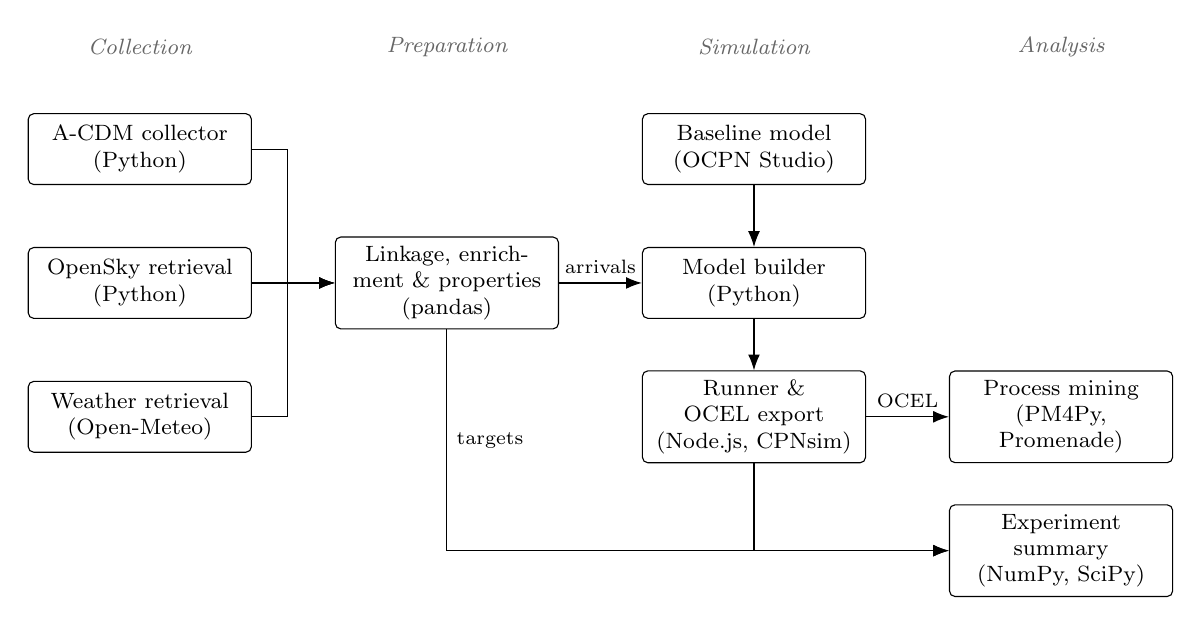
\begin{tikzpicture}[font=\footnotesize,
  box/.style={draw, rectangle, rounded corners=2pt, text width=26mm, minimum height=9mm, align=center},
  lbl/.style={font=\scriptsize},
  hdr/.style={font=\footnotesize\itshape, text=black!60},
  arr/.style={-{Latex[length=2mm]}}]
% column headers
\node[hdr] at (0,2.3) {Collection};
\node[hdr] at (3.9,2.3) {Preparation};
\node[hdr] at (7.8,2.3) {Simulation};
\node[hdr] at (11.7,2.3) {Analysis};
% collection
\node[box] (col) at (0,1.0) {A-CDM collector\\(Python)};
\node[box] (os) at (0,-0.7) {OpenSky retrieval\\(Python)};
\node[box] (wx) at (0,-2.4) {Weather retrieval\\(Open-Meteo)};
% preparation
\node[box] (prep) at (3.9,-0.7) {Linkage, enrichment \& properties\\(pandas)};
% simulation
\node[box] (studio) at (7.8,1.0) {Baseline model\\(OCPN Studio)};
\node[box] (build) at (7.8,-0.7) {Model builder\\(Python)};
\node[box] (run) at (7.8,-2.4) {Runner \&\\OCEL export\\(Node.js, CPNsim)};
% analysis
\node[box] (pm) at (11.7,-2.4) {Process mining\\(PM4Py,\\Promenade)};
\node[box] (exp) at (11.7,-4.1) {Experiment summary\\(NumPy, SciPy)};
% arrows
\draw[arr] (col.east) -- ++(0.45,0) |- (prep.west);
\draw[arr] (os) -- (prep);
\draw[arr] (wx.east) -- ++(0.45,0) |- (prep.west);
\draw[arr] (prep) -- node[lbl,above]{arrivals} (build);
\draw[arr] (studio) -- (build);
\draw[arr] (build) -- (run);
\draw[arr] (run) -- node[lbl,above]{OCEL} (pm);
\draw[arr] (run.south) |- (exp.west);
\draw[arr] (prep.south) -- node[lbl,right]{targets} (prep.south |- exp.west) -- (exp.west);
\end{tikzpicture}
\caption{Implementation components and data flow, from data collection (left) to analysis (right).}
\label{fig:architecture}
\end{figure}

\paragraph{Data collection.}
The A-CDM collector is a Python script that uses only the standard library. A scheduled task starts it every day at 00:15 Berlin time. It requests the departure board of the previous calendar day page by page from the web interface of the BER A-CDM application, with the filter set so that departed flights are included. It checks that every record has an identifier and a scheduled time, removes records that appear twice across pages, and keeps only records whose scheduled departure falls on the requested day. Each raw response is saved together with its SHA-256 hash, and the records are written to a CSV and a JSON table with a reference to the response they come from. An early version of the collector used the application's default filter, which hides departed flights, and returned only six records for 1~November; with the corrected filter the same day contains 289 records. OpenSky arrivals and departures of BER are retrieved through the OpenSky REST interface~\cite{opensky_rest}, and hourly weather through the Open-Meteo archive interface~\cite{openmeteo}.

\paragraph{Linkage and empirical properties.}
The linkage is implemented in Python with pandas. A first script builds one movement table from the OpenSky responses, sorts the movements of each ICAO24 address by time and pairs every arrival with the directly following departure (Section~\ref{sec:method-data}). A second script normalizes the callsigns of both sources and links each A-CDM departure to the OpenSky departure with the same callsign whose first observation lies within 30~minutes of the ATOT; links that are not unique in both directions are discarded. An enrichment script adds the airline (from the callsign), the carrier class (from a lookup table, Appendix~\ref{app:details}), the aircraft type (from A-CDM or the OpenSky aircraft database) and the hourly weather. Every derived table keeps the source file, row and record key of each value. The empirical properties, the held-out delay-transfer model and the early-warning classifiers are computed by separate scripts; the classifiers use scikit-learn~\cite{pedregosa2011sklearn}. Appendix~\ref{app:repro} lists all scripts.

\paragraph{Model builder.}
The model builder is a Python script that reads the unchanged baseline \texttt{.ocpn} file, inserts the arrival list of one day as the initial marking and applies the selected options: timing configuration and calibration multipliers, observed weather, night policy, schedule binding, resource counts, boarding speed and stand-allocation policy. All options are off by default, so that the baseline can be rebuilt exactly. For every model it writes, the builder also records which options were applied.

\paragraph{Headless execution.}
Models are executed with the CPNsim runtime~\cite{cpnsim} in its WebAssembly build (version 0.6.2) from Node.js, without the graphical interface. The runner executes the model until all released turnarounds have departed, then records the per-turnaround timestamps (release, in-block, handling start, service starts and ends, ready, off-block and takeoff) and exports the run as OCEL~2.0. One run of a daily model with about 250 turnarounds takes 45--60~seconds and produces approximately 9,000--10,000 events and 1,100--1,200 objects. Seven runs are executed in parallel, so that a scenario covering all 41 days completes in about five minutes.

\paragraph{Analysis.}
Paired daily contrasts and calibration losses are computed with NumPy, pandas and SciPy. The OCEL logs are analyzed with PM4Py~\cite{berti2023pm4py}. It discovers the OC-DFG and the OCPN and flattens the logs on the \texttt{Turnaround} type. For conformance checking, a Petri net is discovered with the inductive miner (noise threshold 0.2) separately for low-cost and full-service turnarounds, and each net is replayed with token-based replay on the turnarounds of both classes. The calibrated logs of 1, 5 and 8~November and an original-timing log of 8~November are imported into Promenade~\cite{promenade}, where we use the performance spectrum, the process friction topography and the event-log comparison.

\section{Reproducibility}

Each step writes a manifest with input hashes, parameters and output counts. The controlled experiment is defined in a plan file that is fixed before execution, and every run is validated automatically: all released turnarounds must depart, the arrival queue must be empty, all aircraft and resource tokens must have returned to their pools, and all metrics must be finite and nonnegative. The 1,322 A-CDM records, the linked turnarounds and the previous-work dataset are archived together with the scripts that produce every table and figure in Chapter~\ref{ch:evaluation} (Appendix~\ref{app:repro}).

One limitation concerns randomness. The installed CPNsim WebAssembly interface does not expose control of the random seed, so repeating a simulation run produces a new stochastic outcome. We therefore make scenarios comparable through the input instead: every scenario of a day uses the same arrivals and the same weather. How much the remaining randomness changes the results is measured with the Monte Carlo replications described in Section~\ref{sec:method-calibration}; they show a run-to-run variability of at most $\pm1.7$~minutes (Section~\ref{sec:eval-integrity}).

\section{Summary}

The pipeline is implemented as a set of Python and Node.js tools around an unchanged OCPN Studio baseline and the CPNsim runtime. Hashes, manifests and automatic run validation make every result traceable to its inputs. The next chapter uses this implementation to evaluate the approach.

\cleardoublepage
\chapter{Evaluating the Calibrated Simulation at BER}
\label{ch:evaluation}

This chapter evaluates the pipeline on the BER data. It first checks the observations and the empirical properties derived from them, and then uses the simulation to answer the three research questions.

\section{Data Quality and Source Correspondence}
\label{sec:eval-data}

\subsection{Experimental Setup}
The A-CDM collection is checked for completeness per day and for agreement between its CSV, JSON and raw responses. Its actual takeoff times are compared with the OpenSky first observation of the same departure using the linkage rule of Section~\ref{sec:method-data}, under both the UTC and the Europe/Berlin interpretation of the naive A-CDM timestamps.

\subsection{Results}
Table~\ref{tab:acdmcoverage} shows the coverage. All 1,322 records passed the consistency checks. Of the 1,286 eligible actual takeoffs, 1,257 (97.7\%) have a unique OpenSky correspondence, and all of them support the UTC interpretation. The median absolute difference between OpenSky and A-CDM is 8~seconds; 1,237 matches agree within one minute and all 1,257 within five minutes. We therefore interpret the A-CDM timestamps as UTC in all further analyses.

\begin{table}[htbp]\centering\small
\begin{tabular}{lrrr}\hline
Date (2026) & Records & Eligible ATOT & Unique OpenSky match\\\hline
1 November & 289 & 283 & 280\\
5 November & 257 & 251 & 244\\
8 November & 264 & 250 & 243\\
15 November & 254 & 249 & 242\\
16 November & 258 & 253 & 248\\\hline
Total & 1,322 & 1,286 & 1,257\\\hline
\end{tabular}
\caption{A-CDM departure records and OpenSky correspondence per operational day.}
\label{tab:acdmcoverage}
\end{table}

For the 1,283 complete milestone triples, TSAT lies on average 1.30~minutes after TOBT (median 0), and ATOT 12.58~minutes after TSAT (median 12.12). Twenty-two triples violate the expected order $\mathrm{TOBT}\le\mathrm{TSAT}\le\mathrm{ATOT}$; they are retained but flagged. Because the board is retrieved once after the end of the day, only the last value of each target is available, and earlier values that might have respected the order are not.

\section{Empirical Turnaround Properties, Delay Drivers and Early Warning}
\label{sec:eval-props}

\subsection{Experimental Setup}
P1 and P2 are computed on the 610 linked turnarounds and P3 and P4 on the 1,283 complete departures. Associations are measured by Spearman's $\rho$ with 95\% bootstrap intervals from 5,000 resamples. The held-out delay-transfer model and the delay-driver models use the February--April data; the early-warning classifiers use both datasets (Section~\ref{sec:method-targets}).

\subsection{P1: Buffer-Dependent Delay Transfer}
When the inbound aircraft lands 30~minutes or less before the scheduled departure, the operator sets the TOBT more than five minutes after STD in 99\% of the cases, with a median shift of 35~minutes (Table~\ref{tab:p1}). Between 30 and 45~minutes of buffer this share falls to 53\%, and above 45~minutes it stays between 14\% and 26\%. The rank correlation between buffer and target shift is $\rho=-0.54$ (95\% CI $[-0.60,-0.46]$), and it is stable across days ($-0.52$, $-0.57$ and $-0.54$ on 1, 5 and 8~November).

\begin{table}[htbp]\centering\small
\begin{tabular}{lrrr}\hline
Scheduled buffer $B$ & $n$ & TOBT $>$ STD $+5$\,min & Median $\Delta^{\mathrm{TOBT}}$ (min)\\\hline
$\le 30$ min & 88 & 99\% & 35.0\\
30--45 min & 90 & 53\% & 7.5\\
45--60 min & 216 & 26\% & 0.0\\
60--90 min & 159 & 23\% & 0.0\\
$>90$ min & 57 & 14\% & 0.0\\\hline
\end{tabular}
\caption{P1: share of linked turnarounds with a late target off-block time by scheduled buffer, $n=610$.}
\label{tab:p1}
\end{table}

\subsection{P2: Target Turnaround Time}
The target turnaround time from the landing proxy to the TOBT differs clearly between carrier classes (Table~\ref{tab:p2}). Under time pressure, low-cost carriers plan turnarounds of 33.7~minutes or less in 5\% of the cases, full-service carriers 37.1~minutes. These distributions are the calibration targets of Section~\ref{sec:eval-rq1}.

\begin{table}[htbp]\centering\small
\begin{tabular}{llrrrr}\hline
Carrier class & Buffer & $n$ & 5th pct. & 25th pct. & Median\\\hline
Low-cost & $<45$ min & 113 & 33.7 & 39.7 & 44.7\\
Low-cost & $\ge45$ min & 163 & 41.9 & 51.3 & 61.0\\
Full-service/other & $<45$ min & 65 & 37.1 & 44.6 & 52.3\\
Full-service/other & $\ge45$ min & 269 & 47.7 & 55.4 & 64.0\\\hline
\end{tabular}
\caption{P2: target turnaround time (landing proxy to TOBT, minutes) by carrier class and schedule pressure.}
\label{tab:p2}
\end{table}

\subsection{P3 and P4: Runway Contention and Rotation Carry-Over}
The interval from start-up approval to takeoff grows with the number of other departures planned around the same time, from a median of 10.2~minutes with at most two others within $\pm15$~minutes ($n=27$) to 12.9~minutes with more than eight ($n=632$; $\rho=0.14$, CI $[0.08,0.19]$). In 154 cases, the same aircraft departed BER twice on one day; the departure delays of the two flights are positively associated ($\rho=0.27$, CI $[0.11,0.42]$).

\subsection{Delay Drivers and Weather}
On the February--April data, the outbound delay increases by 0.43~minutes per minute of inbound delay (95\% day-resampled CI $[0.13,0.62]$), and an inbound delay of more than 15~minutes doubles the odds of an outbound delay above 15~minutes (odds ratio 2.10, CI $[1.18,3.17]$). Low-cost turnarounds have lower odds of a late departure than full-service turnarounds (odds ratio 0.74, CI $[0.56,0.97]$), although their scheduled ground times are shorter (median 110 versus 145~minutes).

Weather shows the expected direction, but the evidence is weak. With precipitation at landing, 56\% of departures are more than 15~minutes late, compared with 45\% in dry conditions (median delay 18 versus 14~minutes). All eight turnarounds with gusts of 50~km/h or more departed late (median 36~minutes). In the multivariable model, however, the odds ratios for precipitation (1.25, CI $[0.72,2.95]$) and gusts of 40~km/h or more (3.09, with an unbounded upper limit) are not distinguishable from one, because the data cover only 20 days and few weather events. No de-icing conditions occurred in the observed periods.

\subsection{Held-Out Delay-Transfer Model}
Table~\ref{tab:heldout} reports the reactionary-delay model of Equation~\ref{eq:transfer}. On the April test data it is clearly better than assuming full transfer of the inbound delay, but it does not outperform a constant prediction. Only 9.8\% (full-service) and 16.5\% (low-cost) of the test turnarounds exceed the estimated slack, so the minimum turnaround time is poorly identified. Together with P1, this shows that inbound delay is transferred mainly when the buffer is short; with the long scheduled ground times of this sample, most outbound delay arises at BER itself.

\begin{table}[htbp]\centering\footnotesize
\begin{tabular}{lrrrrrr}\hline
& & & \multicolumn{3}{c}{Test MAE (min)} & \\\cline{4-6}
Class & $n_{\mathrm{train}}/n_{\mathrm{test}}$ & MTT [95\% CI] & Model & Full transf. & Const. & Slack exc.\\\hline
Full-service & 1,094 / 305 & 70 [20, 90] & 17.5 & 21.1 & 16.3 & 9.8\%\\
Low-cost & 390 / 278 & 62 [37, 80] & 18.7 & 22.9 & 18.2 & 16.5\%\\\hline
\end{tabular}
\caption{Held-out evaluation of the delay-transfer model (Eq.~\ref{eq:transfer}), trained on 21~February--4~March and tested on 17--24~April~2026.}
\label{tab:heldout}
\end{table}

\subsection{Early Warning at Landing}
Table~\ref{tab:earlywarning} shows that a late TOBT can be detected when the inbound aircraft lands. On each held-out November day, the classifiers reach an AUC between 0.76 and 0.82. When as many turnarounds are flagged as are actually late, 59--70\% of the flagged turnarounds are indeed late, compared with base rates of 33--48\%. The scheduled buffer is by far the most important feature (mean permutation importance 0.28 AUC), followed by temperature (0.02) and hour (0.01); the remaining weather variables, the carrier class and the arrival load contribute little. The median lead time, the scheduled buffer itself, is 54~minutes.

\begin{table}[htbp]\centering\footnotesize
\begin{tabular}{lrrrr}\hline
Test day & Base rate & AUC (logistic) & AUC (trees) & Precision\\\hline
1 November & 0.48 & 0.80 & 0.81 & 0.70\\
5 November & 0.33 & 0.82 & 0.76 & 0.59\\
8 November & 0.34 & 0.79 & 0.80 & 0.65\\\hline
Feb--Apr data (test April) & 0.35 & 0.54 & 0.53 & 0.42\\\hline
\end{tabular}
\caption{Early detection of delays at landing. November 2026: late TOBT, leave-one-day-out. February--April: outbound delay above 15 minutes, trained on February--March. Trees: gradient-boosted trees. Precision of the boosted trees when as many turnarounds are flagged as are actually late (base rate).}
\label{tab:earlywarning}
\end{table}

On the February--April data, predicting the actual outbound delay at landing does not work (AUC 0.53--0.54). The actual delay depends on events after landing that these features do not capture, and the flight-number pairing may join flights that are not true rotations. Early warning is therefore feasible for the \emph{planned} target, which depends strongly on the buffer, but not yet for the \emph{actual} departure delay.

\subsection{Disruption Screening}
Screening the 41 days of OpenSky turnarounds against a season- and weekday-specific baseline flags 15--17 and 20~October, when the median ground time of short stays was about 5--9~minutes above normal ($z$ between 3.2 and 5.6). These days were dry and calm (maximum gusts below 35~km/h), so weather does not explain them. They coincide with the start of the Berlin and Brandenburg autumn school holidays on 19~October~\cite{herbstferien2026}, when fuller flights and more baggage can lengthen turnarounds. In early November, the screening also flags a day with low traffic (8~November) and one with long ground times (9~November), but the winter-schedule baseline contains only 16 days and is less reliable. Larger disruptions, such as the warning strike that closed BER on 18~March~2026~\cite{aerointernational2026streik}, fall outside the collected periods; with no turnarounds at all, such a day would be flagged immediately.

\section{Simulation Integrity and Run-to-Run Variability}
\label{sec:eval-integrity}

All 499 simulation runs reported in this chapter (three timing configurations and six what-if scenarios on 41 days, the 116 runs of the calibration grid and 14 validation runs on the held-out days) completed and passed the automatic checks: every released turnaround departed, all aircraft and resource tokens returned to their pools, and all metrics were finite and nonnegative. The exported logs contain no dangling event-to-object or object-to-object references. One modeling artefact remains: some resource objects are related to service events twice, once with the qualifier of the resource and once with the qualifier \texttt{turnaround}.

The Monte Carlo comparison quantifies how much a single run of a day can vary. With ten independent replications per scenario on 1 and 8~November, the 95\% interval of the mean block duration is between $\pm0.3$ and $\pm1.7$~minutes. This is small compared with the effects studied below and with the variation between days, which justifies single trace-driven runs per day and the use of the day as the statistical unit.

\section{RQ1: Calibration of Service Times}
\label{sec:eval-rq1}
\label{sec:eval-validity}

\subsection{Experimental Setup}
For every linked turnaround, the simulated time from arrival release to \emph{Aircraft Ready} is compared with the observed target turnaround time (P2). We first compare the three timing configurations on all 41 days, then calibrate the carrier-specific configuration (Section~\ref{sec:method-calibration}).

\subsection{Timing Configurations}
Table~\ref{tab:timingconfig} shows that the carrier-specific service times reproduce the observed targets far better than the original and the carrier-agnostic literature functions. For low-cost turnarounds, the mean quantile error drops from 13.5~minutes (original) and 10.6~minutes (literature) to 5.8~minutes; for full-service turnarounds from 10.8 and 4.5~minutes to 3.8~minutes. The comparison also revealed that leisure carriers do not behave like low-cost carriers: their observed target turnaround is long (median 79.8~minutes), and the low-cost profile underestimates it by more than 27~minutes. Leisure carriers therefore use the full-service profile in the calibrated model.

\begin{table}[htbp]\centering\small
\begin{tabular}{lrrr}\hline
Mean quantile error (min) & Original & Literature & Carrier-specific\\\hline
Full-service ($n=259$) & 10.8 & 4.5 & 3.8\\
Low-cost ($n=266$) & 13.5 & 10.6 & 5.8\\
Leisure ($n=52$), low-cost profile & 10.8 & 13.8 & 27.7\\\hline
\end{tabular}
\caption{Mean absolute difference of the 5th, 25th, 50th and 75th percentiles between simulated arrival-to-ready time and observed target turnaround time, linked turnarounds, one run per day.}
\label{tab:timingconfig}
\end{table}

\subsection{Calibration and Held-Out Validation}
The grid search places the optimum at $s_{\mathrm{LCC}}=1.3$ and $s_{\mathrm{FSC}}=1.1$ (calibration loss 2.03~minutes, compared with 4.84~minutes without calibration). Neighbouring values are clearly worse, and extending the grid to $s_{\mathrm{LCC}}=1.6$ confirmed that the optimum is interior. The literature service times are therefore slightly too fast for BER, by about 30\% for low-cost and 10\% for full-service turnarounds.

The calibration is validated on three held-out days that were not used for fitting: 8~November and the two most recent collection days, 15 and 16~November. The latter lie outside the frozen 41-day period; their 437 turnarounds were reconstructed from the raw OpenSky lists with the same pairing rule and linked to A-CDM in the same way (372 linked low-cost and full-service turnarounds). Table~\ref{tab:calibration} compares the calibrated model with the uncalibrated carrier timing, the carrier-agnostic literature timing and the original timing.

On 8~November, calibration reduces the loss from 8.55 to 2.39~minutes. The simulated low-cost quartiles move from $[36.8, 44.9, 53.3]$ to $[43.1, 52.1, 59.8]$~minutes against observed $[44.5, 52.6, 66.1]$, and the full-service quartiles from $[45.3, 55.2, 67.6]$ to $[51.9, 60.6, 72.6]$ against observed $[55.3, 63.1, 72.9]$. On 15--16~November the reduction is smaller, from 6.05 to 3.85~minutes. Here the full-service turnarounds are reproduced closely (median 59.4 against 59.1~minutes), but the low-cost turnarounds remain about six minutes too fast at the 25th and 50th percentiles.

The comparison with the literature timing is more nuanced. On 8~November the calibrated model is clearly better (2.39 against 6.59~minutes), whereas on 15--16~November both reach the same overall loss (3.85 and 3.82). The errors have opposite signs: the carrier-agnostic literature timing makes low-cost turnarounds too \emph{slow} on all three days (by 4 to 14~minutes per quartile), while the calibrated model makes them slightly too \emph{fast} on 15--16~November. Averaged over the two held-out sets, the calibrated model has the lowest loss (3.1~minutes, against 5.2 for literature, 7.3 for uncalibrated and 8.7 for original timing). The calibration therefore generalizes in direction and order of magnitude, while the remaining differences of a few minutes between days are larger than the run-to-run variability (Section~\ref{sec:eval-integrity}) and indicate genuine day-to-day variation in the planned turnaround times.

\begin{table}[htbp]\centering\small
\begin{tabular}{llccr}\hline
Held-out day(s) & Source & Low-cost quartiles & Full-service quartiles & Loss\\\hline
8 Nov. & observed TTA & $[44.5, 52.6, 66.1]$ & $[55.3, 63.1, 72.9]$ & \\
 & calibrated & $[43.1, 52.1, 59.8]$ & $[51.9, 60.6, 72.6]$ & \textbf{2.39}\\
 & uncalibrated & $[36.8, 44.9, 53.3]$ & $[45.3, 55.2, 67.6]$ & 8.55\\
 & literature & $[52.4, 66.2, 76.1]$ & $[49.0, 63.1, 74.6]$ & 6.59\\
 & original & $[57.4, 67.3, 85.2]$ & $[57.4, 73.0, 82.8]$ & 11.43\\\hline
15--16 Nov. & observed TTA & $[44.0, 51.3, 65.4]$ & $[52.0, 59.1, 68.5]$ & \\
 & calibrated & $[38.3, 45.5, 61.4]$ & $[47.2, 59.4, 71.1]$ & 3.85\\
 & uncalibrated & $[36.0, 47.7, 56.0]$ & $[44.6, 53.9, 65.7]$ & 6.05\\
 & literature & $[48.7, 59.1, 69.8]$ & $[47.6, 58.8, 67.2]$ & \textbf{3.82}\\
 & original & $[49.9, 58.8, 67.7]$ & $[57.0, 67.4, 75.5]$ & 6.02\\\hline
\end{tabular}
\caption{Held-out validation of the calibration (minutes; 25th, 50th and 75th percentiles of the target turnaround time). 8~November: 88 low-cost and 100 full-service linked turnarounds; 15--16~November: 174 and 198.}
\label{tab:calibration}
\end{table}

\subsection{Validation on the 41-Day Demand}
On all 41 days, the calibrated model also reproduces the ground intervals of the 10,212 OpenSky turnarounds at the lower and middle quantiles. For short stays of full-service aircraft, the simulated 25th and 50th percentiles of the arrival-to-takeoff time are 64.1 and 75.6~minutes against observed 64.2 and 71.6; for low-cost aircraft 56.0 and 65.6 against 57.2 and 66.6. The original timing overestimates these quantiles by 10 to 14~minutes. The upper tail is not reproduced, because most simulated aircraft without a linked schedule depart as soon as they are ready.

Figure~\ref{fig:p1sim} compares the simulated delay-transfer curve with the observed one. Under schedule binding, the simulated share of late targets equals $\max(0,\mathrm{ready}-\mathrm{STD})>5$~minutes. The calibrated model reproduces the observed transfer at short buffers and moves the 30--45-minute class from 99\% (original) to 78\% (observed 54\%). It still transfers too much delay at intermediate buffers, because it does not compress turnarounds under pressure.

\begin{figure}[htbp]
\centering
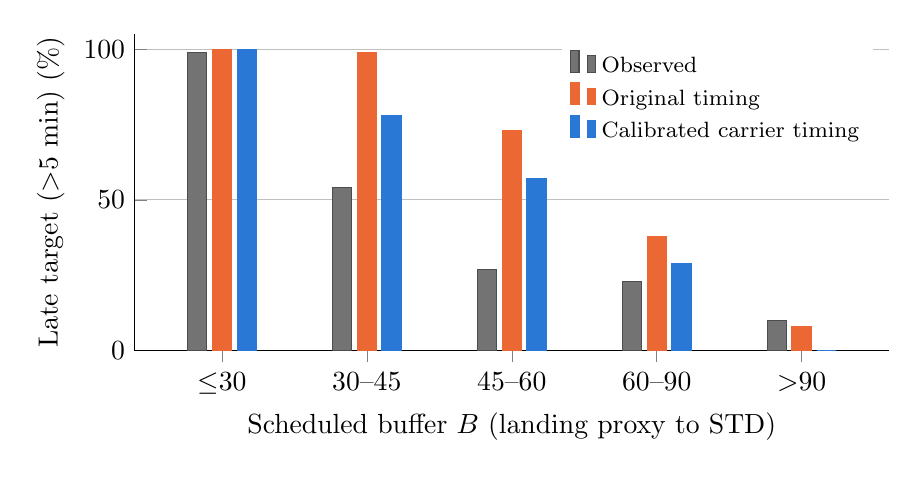
\begin{tikzpicture}
\begin{axis}[
  ybar, bar width=7pt, width=0.92\textwidth, height=5.6cm,
  ymin=0, ymax=105, ylabel={Late target ($>$5 min) (\%)},
  xlabel={Scheduled buffer $B$ (landing proxy to STD)},
  symbolic x coords={{$\le$30},{30--45},{45--60},{60--90},{$>$90}},
  xtick=data, enlarge x limits=0.15, axis lines*=left, ymajorgrids,
  legend style={at={(0.98,0.97)}, anchor=north east, font=\footnotesize, draw=none}, legend cell align=left]
\addplot[fill=black!55, draw=black!70] coordinates {({$\le$30},99) ({30--45},54) ({45--60},27) ({60--90},23) ({$>$90},10)};
\addplot[fill={rgb,255:red,235;green,104;blue,52}, draw={rgb,255:red,235;green,104;blue,52}] coordinates {({$\le$30},100) ({30--45},99) ({45--60},73) ({60--90},38) ({$>$90},8)};
\addplot[fill={rgb,255:red,42;green,120;blue,214}, draw={rgb,255:red,42;green,120;blue,214}] coordinates {({$\le$30},100) ({30--45},78) ({45--60},57) ({60--90},29) ({$>$90},0)};
\legend{Observed, Original timing, Calibrated carrier timing}
\end{axis}
\end{tikzpicture}
\caption{Observed and simulated delay-transfer curves (P1) for the linked turnarounds.}
\label{fig:p1sim}
\end{figure}

\section{RQ2: Waiting, Synchronization and Delay Propagation}
\label{sec:eval-promenade}

\subsection{Experimental Setup}
We analyze the calibrated reference runs of all 41 days by carrier class and stand type, and the calibrated event logs of 1, 5 and 8~November with PM4Py and Promenade (Section~\ref{sec:method-ocel}).

\subsection{Which Branch Determines Readiness}
Table~\ref{tab:mechanism} shows which handling branch finishes last at the join. For full-service turnarounds, the cabin and boarding branch is last in 86\% of the cases. For low-cost turnarounds, whose cabin services are shorter, it is last in only 76\%, and the baggage hold becomes the critical branch in 13\% of the cases, compared with 3\% for full-service. Faster cabin processes thus shift the bottleneck to the ramp.

\begin{table}[htbp]\centering\small
\begin{tabular}{lrrrrr}\hline
Class & Turnarounds & Cabin/boarding & Baggage hold & Fuel & Other\\\hline
Full-service & 3,993 & 86.2\% & 3.4\% & 8.7\% & 1.7\%\\
Leisure & 928 & 87.2\% & 2.4\% & 9.2\% & 1.2\%\\
Low-cost & 4,963 & 76.4\% & 12.9\% & 6.8\% & 3.9\%\\\hline
Contact stands & & 70.8\% & 12.7\% & 12.0\% & 4.5\%\\
Remote stands & & 99.0\% & 0.0\% & 1.0\% & 0.0\%\\\hline
\end{tabular}
\caption{Last-ready handling branch in the calibrated reference runs (41 days), by carrier class and stand type.}
\label{tab:mechanism}
\end{table}

\subsection{Terminal and Remote Stands}
Remote stands, which receive 38\% of the turnarounds in the model, add 18.5~minutes to the time until the aircraft is ready (paired daily difference, 95\% CI $[17.0,20.0]$) and 17.8~minutes to the block time ($[16.3,19.3]$). On remote stands, deplaning and boarding by bus make the cabin branch the last-ready branch in 99\% of the turnarounds; on contact stands, the bottleneck is spread over cabin (71\%), baggage (13\%) and fuel (12\%). Within each carrier class, the median ready time is about 19~minutes longer on a remote stand (low-cost 59.3 versus 40.9~minutes, full-service 68.6 versus 48.9~minutes). These values describe the mechanism, not BER's actual remote-stand penalty. BER does not publish its stand layout, the walking and driving distances to its remote stands or the size of its bus fleet, so the model keeps the stand geometry and the bus fleet of the generic baseline airport. The size of the penalty therefore depends on these inherited assumptions, while its cause, bus transport on the cabin branch, does not.

\subsection{Object-Centric Process Discovery}
The calibrated log of 8~November contains 8,914 events, 1,104 objects and 47 activities. Figure~\ref{fig:ocdfg} shows the OC-DFG restricted to the shared resources. Each color stands for one resource type, each node for an activity, and each edge for a directly-follows relation of objects of that type, labeled with how often it occurs. Unlike a turnaround, a resource object does not have a single start and end: it returns to an earlier activity when it serves the next aircraft, so its edges form cycles. The figure makes the lifecycle of each resource across turnarounds visible: pushback tugs cycle through \emph{attached}, \emph{start-up} and \emph{off-block}; fuel tankers alternate between \emph{dispatch}, \emph{refuelling} and, 30 times on this day, \emph{reload at depot}; buses run deplaning and boarding cycles; and loaders move between unloading and loading of different aircraft. None of these cycles is visible in a case-centric log of turnarounds.

\begin{figure}[htbp]\centering
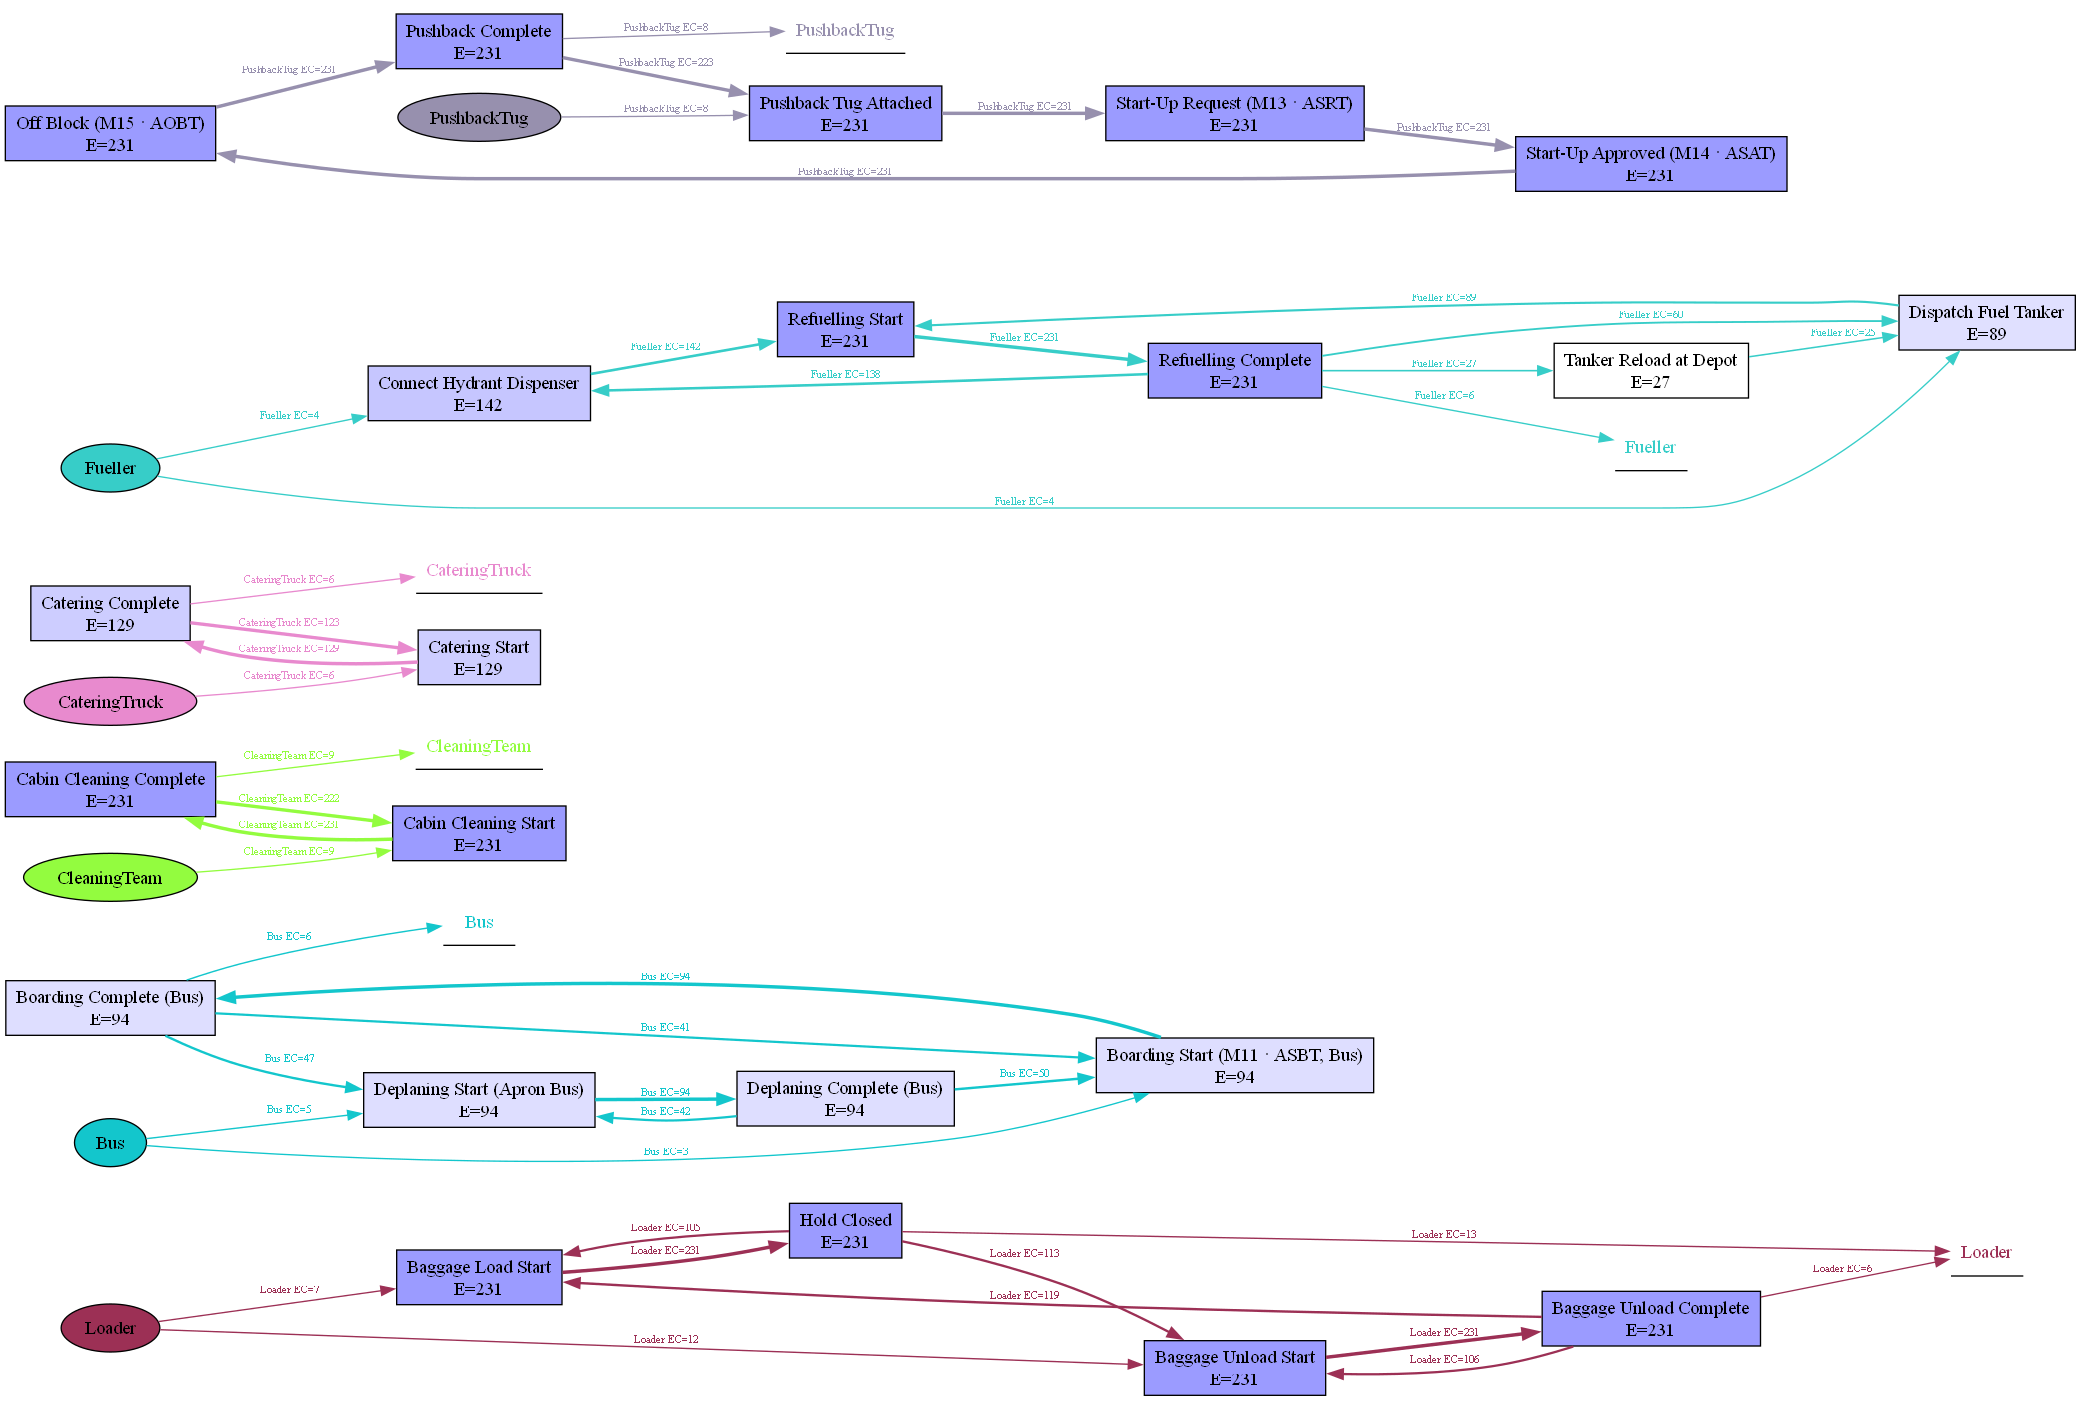
\includegraphics[width=\textwidth]{pm_ocdfg_resources.png}
\caption{OC-DFG of the shared resource types discovered with PM4Py from the calibrated log of 8 November (edge labels: event couples).}
\label{fig:ocdfg}
\end{figure}

The discovered OCPN (Figure~\ref{fig:ocpn}) shows the turnaround in brown and three resource types in color: fuel tankers and buses in cyan and cleaning teams in green. Read from top to bottom, the brown part recovers the sequential parts of the turnaround (approach, in-block, pushback, taxi-out), and the colored parts at the bottom recover the resource cycles. The parallel handling between \emph{Start Ground Handling} and \emph{Aircraft Ready}, however, is represented as a single place in the middle of the figure from which all handling activities can occur in any order and any number of times (a so-called flower structure). The reason is concurrency: among 383 full-service and 330 low-cost turnarounds of the three days, 381 and 318 have a unique order of activities, so the inductive miner finds no order that holds for all of them.

\begin{figure}[htbp]\centering
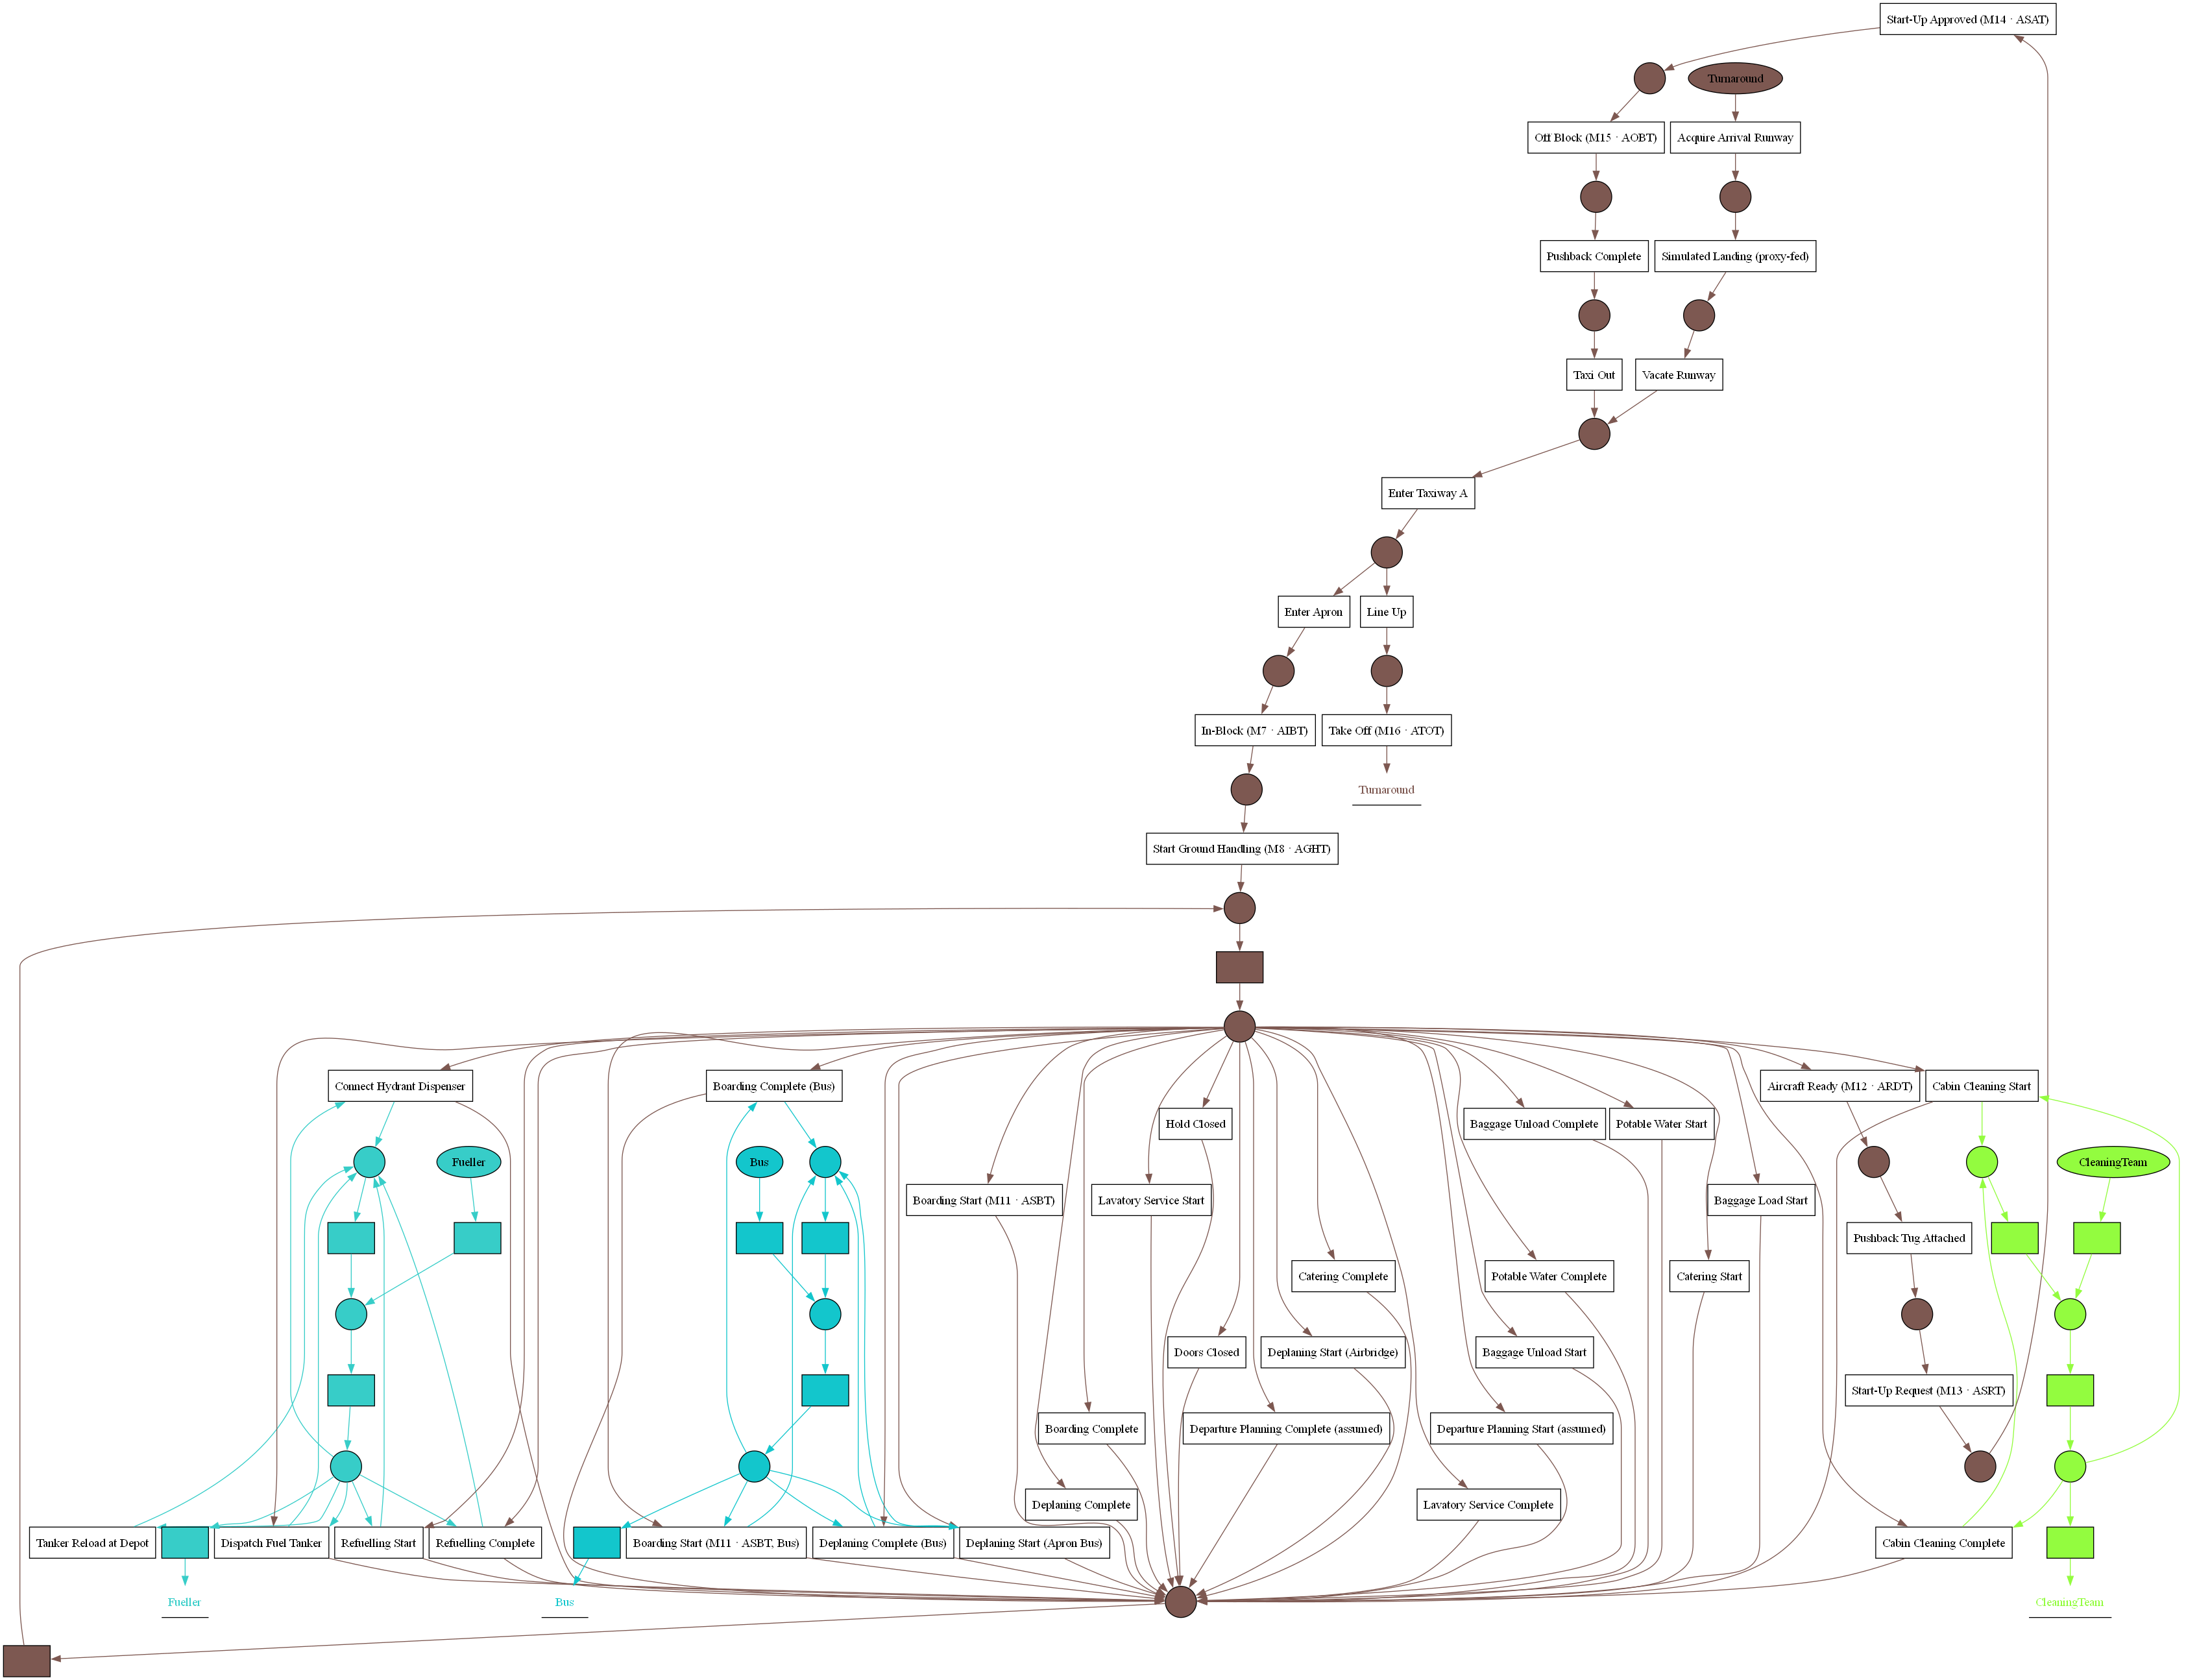
\includegraphics[width=\textwidth]{pm_ocpn.png}
\caption{OCPN discovered with PM4Py (inductive miner) for the object types Turnaround, Fueller, Bus and CleaningTeam.}
\label{fig:ocpn}
\end{figure}

\subsection{Carrier-Specific Behavior in the Event Logs}
Flattening the logs on the turnaround object confirms the carrier differences at the level of the individual services (Table~\ref{tab:pmdurations}). Cleaning, catering and boarding take 5--7~minutes less for low-cost turnarounds, and the median ground handling from its start to \emph{Aircraft Ready} is 36.2 versus 48.6~minutes.

\begin{table}[htbp]\centering\small
\begin{tabular}{lrrrr}\hline
Service (median, min) & Full-service & Low-cost & Full p90 & Low p90\\\hline
Deplaning & 7.5 & 8.1 & 16.3 & 17.2\\
Cleaning & 15.5 & 10.1 & 21.5 & 16.2\\
Catering & 18.3 & 11.6 & 29.6 & 16.4\\
Refuelling & 14.2 & 14.8 & 34.6 & 23.9\\
Boarding & 20.2 & 14.0 & 29.7 & 23.6\\
Ground handling (start to ready) & 48.6 & 36.2 & 65.0 & 55.0\\\hline
\end{tabular}
\caption{Service durations measured in the flattened calibrated logs (1, 5 and 8 November; 383 full-service and 330 low-cost turnarounds), including access and travel times.}
\label{tab:pmdurations}
\end{table}

Conformance checking makes the behavioral difference measurable. A natural reference would be the de-jure model, that is, the simulation model itself. Since every generated trace is produced by that model, replaying the logs on it would trivially yield perfect fitness and would show nothing. We therefore use the two carrier classes as references for each other: a model discovered from one class is replayed on the traces of both classes, and the fit on its own class serves as the baseline for the fit on the other class (Table~\ref{tab:conformance}). A Petri net discovered from low-cost turnarounds replays 82.7\% of the low-cost traces perfectly but only 65.5\% of the full-service traces; the net discovered from full-service turnarounds replays 61.4\% of full-service and 46.7\% of low-cost traces. Log fitness stays high (0.98--1.00) in all cases, whereas precision is low (0.26--0.29) because the discovered nets allow the parallel activities in any order.

\begin{table}[htbp]\centering\small
\begin{tabular}{llrrr}\hline
Model discovered from & Replayed log & Fitness & Perfectly fitting traces & Precision\\\hline
Low-cost & Low-cost & 0.997 & 82.7\% & 0.26\\
Low-cost & Full-service & 0.993 & 65.5\% & 0.26\\
Full-service & Full-service & 0.991 & 61.4\% & 0.29\\
Full-service & Low-cost & 0.984 & 46.7\% & 0.28\\\hline
\end{tabular}
\caption{Token-based replay conformance between carrier classes (flattened calibrated logs, inductive miner with noise threshold 0.2).}
\label{tab:conformance}
\end{table}

\subsection{Analysis in Promenade}
\todo[inline]{Figs.~6.4 and 6.5: retake the Promenade screenshots in light mode and crop them to the relevant part (supervisor comment).}
The Promenade performance spectrum of the calibrated 8~November log (Figure~\ref{fig:spectrum}) shows the slowest 25\% of flows concentrated in three segments: the wait from \emph{Aircraft Ready} to the start-up request of aircraft held to their schedule, the transition from baggage unloading to loading, and a departure that the night restriction holds until the morning. The process friction topography (Figure~\ref{fig:friction}), which raises each activity by its median waiting time, places its summit at \emph{Hold Closed} with a median queue of 4.7~minutes. This confirms the baggage hold as the main point of friction in the calibrated model.

\begin{figure}[htbp]\centering
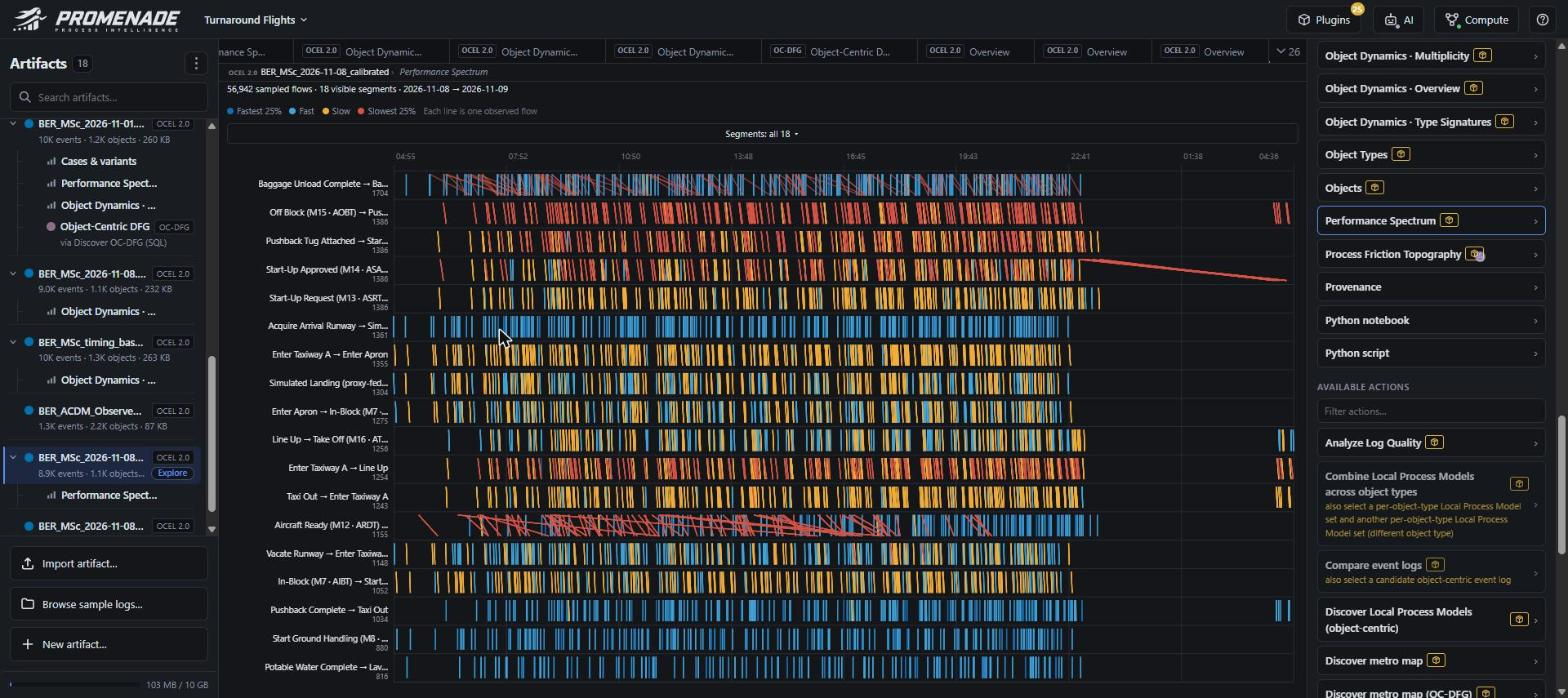
\includegraphics[width=\textwidth]{promenade_performance_spectrum.jpg}
\caption{Promenade performance spectrum of the calibrated log of 8 November (blue: fastest flows, red: slowest 25\%).}
\label{fig:spectrum}
\end{figure}

\begin{figure}[htbp]\centering
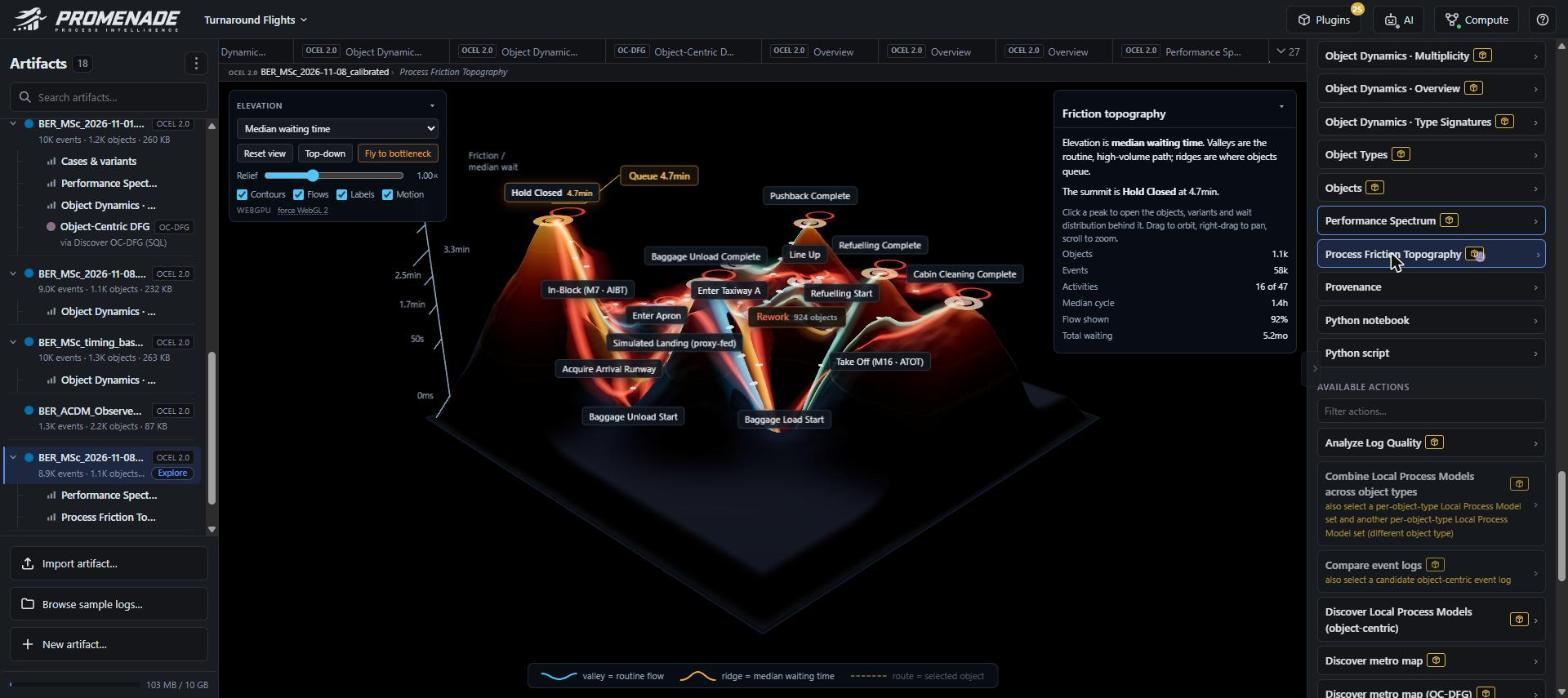
\includegraphics[width=\textwidth]{promenade_friction_topography.jpg}
\caption{Promenade process friction topography of the calibrated log of 8 November; elevation is the median waiting time.}
\label{fig:friction}
\end{figure}

Finally, Promenade's event-log comparison between the calibrated and the original-timing log of the same day finds identical behavior and objects at the type level: all 47 activity types are shared, and 94.5\% of the objects. Only 63.7\% of the events coincide, because their timestamps differ. Calibration thus changes \emph{when} the services happen, not \emph{which} services happen.

\subsection{Delay Propagation in the Simulation}
Delay propagates in the model through the same three channels as in the observations: through the turnaround, as the simulated transfer curve shows (Figure~\ref{fig:p1sim}); through the aircraft, whose token is reused in later rotations of the day, as the running example shows; and through shared resources, whose queues (fuel dispatch, pushback tugs) delay the branches that use them. The object-centric view separates waiting that matters from waiting that does not: an aircraft can wait for fuel without any effect on its readiness if its cabin branch finishes later.

\section{RQ3: Resource and Allocation Scenarios}
\label{sec:eval-whatif}

\subsection{Experimental Setup}
The calibrated model is run on all 41 days for the reference and five scenarios (Section~\ref{sec:method-calibration}). Effects are paired daily differences with 95\% Student-$t$ intervals over 41 days.

\subsection{Results}
Table~\ref{tab:whatif} and Figure~\ref{fig:whatif} summarize the effects on the time from arrival to \emph{Aircraft Ready}, whose reference mean is 58.7~minutes. Faster boarding is the most effective single lever: a 15\% reduction of boarding time shortens the time to readiness by 2.2~minutes and the block time by 1.5~minutes, and it benefits full-service turnarounds most ($-2.6$~minutes), because their cabin branch is critical more often. Additional fuel capacity removes almost the whole fuel queue ($-2.5$~minutes of dispatch waiting) but shortens the time to readiness by only 1.3~minutes, more for low-cost ($-1.8$) than for full-service turnarounds. Four additional buses shorten the time to readiness by about half a minute, and five additional loaders do not change it; for both, the confidence interval includes zero.

\begin{table}[htbp]\centering\footnotesize\setlength{\tabcolsep}{4pt}
\begin{tabular}{lrrr}\hline
Scenario (vs.\ calibrated reference) & Ready (min) & Block (min) & Fuel wait (min)\\\hline
Boarding 15\% faster & $-2.17$ [$-2.85$, $-1.49$] & $-1.50$ [$-2.06$, $-0.94$] & $+0.30$ [$-0.12$, $+0.71$]\\
Fuel 6+6 instead of 4+4 & $-1.35$ [$-2.10$, $-0.59$] & $-0.86$ [$-1.49$, $-0.22$] & $-2.47$ [$-2.83$, $-2.10$]\\
Buses 12 instead of 8 & $-0.56$ [$-1.19$, $+0.08$] & $-0.46$ [$-1.09$, $+0.16$] & $-0.29$ [$-0.64$, $+0.06$]\\
Loaders 24 instead of 19 & $-0.02$ [$-0.66$, $+0.63$] & $-0.19$ [$-0.80$, $+0.41$] & $+0.18$ [$-0.22$, $+0.58$]\\
Low-cost to remote stands & $+37.9$ [$+31.1$, $+44.7$] & $+7.1$ [$+5.4$, $+8.7$] & $-0.63$ [$-0.96$, $-0.30$]\\\hline
\end{tabular}
\caption{What-if effects: paired daily differences over 41 days with 95\% intervals.}
\label{tab:whatif}
\end{table}

\begin{figure}[htbp]
\centering
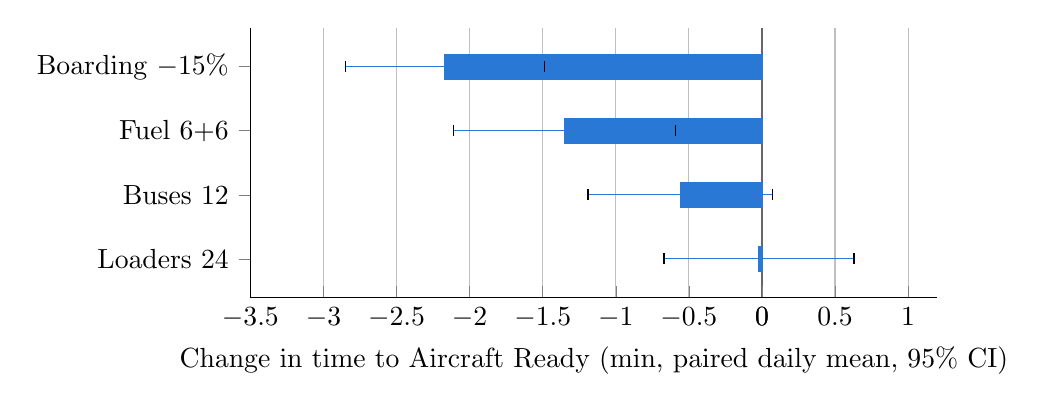
\begin{tikzpicture}
\begin{axis}[
  xbar=0pt, width=0.85\textwidth, height=5.0cm, xmin=-3.5, xmax=1.2,
  xlabel={Change in time to Aircraft Ready (min, paired daily mean, 95\% CI)},
  symbolic y coords={Loaders 24,Buses 12,Fuel 6+6,Boarding $-$15\%}, ytick=data,
  axis lines*=left, xmajorgrids, bar width=9pt, enlarge y limits=0.2,
  extra x ticks={0}, extra x tick style={grid=major, major grid style={black!60}}]
\addplot[fill={rgb,255:red,42;green,120;blue,214}, draw={rgb,255:red,42;green,120;blue,214},
  error bars/.cd, x dir=both, x explicit]
  coordinates {(-0.02,Loaders 24) +- (0.65,0) (-0.56,Buses 12) +- (0.63,0) (-1.35,Fuel 6+6) +- (0.76,0) (-2.17,Boarding $-$15\%) +- (0.68,0)};
\end{axis}
\end{tikzpicture}
\caption{Effects of capacity and process scenarios on the time to readiness. The allocation scenario (+37.9 min) is omitted for scale.}
\label{fig:whatif}
\end{figure}

The allocation strategy that sends all low-cost turnarounds to remote stands is clearly harmful in the modeled airport. Full-service turnarounds gain 9.0~minutes ($[-11.2,-6.8]$) from the freed contact stands, but low-cost aircraft wait for a free remote stand and need 86.8~minutes longer ($[73.3,100.3]$) until they are ready. The remote apron of the model is not large enough for the low-cost share of BER's demand. The strategy would only be viable with more remote stands or a flexible assignment that uses contact stands when the remote apron is full.

\section{Threats to Validity}
\label{sec:threats}

The results of this chapter rest on observations that were not collected for this purpose and on a model that was not built for BER. Both limit what the results can show. We discuss the threats in the order of the pipeline, from the data to the model and its runs.

The first threat concerns what the data measure. OpenSky's last observation of an arriving aircraft is only a proxy for its landing, and the A-CDM board is retrieved once after the end of the day, so only the last value of each target is available. The calibration therefore matches \emph{planned} turnaround times (TOBT) rather than actual ones, and these times include taxi-in. The data also contain few weather events and no de-icing conditions, so weather effects could not be estimated precisely, and the disruption screening relies on a short baseline. The carrier classification is based on business models, and the February--April records pair flights by flight number rather than by aircraft.

The second threat concerns the calibration. It uses two days and is validated on three held-out days with 560 linked turnarounds. On 15--16~November it does not improve on the carrier-agnostic literature timing, and low-cost turnarounds are simulated too fast. Leisure carriers ($n=52$) remain poorly reproduced (mean quantile error 11.8~minutes). The carrier-specific distributions themselves were measured at other airports and are scaled, not re-estimated, for BER, because individual service durations at BER are not observed.

The third threat concerns the model and its runs. Stand geometry and the bus, loader and fuel fleets are inherited from the generic airport model, because BER's infrastructure data are not public. Absolute effects of capacity and stand scenarios are therefore model-specific; their direction and relative size are the transferable result. Finally, each scenario is run once per day. The Monte Carlo comparison shows that the run-to-run variability is small, but individual days remain single realizations.

\section{Summary}

The evaluation shows that public milestones, once linked to arrival observations, reveal systematic properties of BER turnarounds and allow an early warning at landing with an AUC of about 0.8. Carrier-specific service times reproduce the observed targets far better than carrier-agnostic ones, and calibrating them by 30\% (low-cost) and 10\% (full-service) reduces the error on three held-out days by 36--72\%. The object-centric analysis shows that the cabin branch determines readiness for most turnarounds, that the baggage hold becomes critical for low-cost turnarounds, and that remote stands add almost 20~minutes. Process discovery and conformance checking make the carrier differences measurable in the event logs. Among the tested levers, faster boarding is most effective, additional fuel capacity mainly removes the fuel queue, and assigning all low-cost flights to remote stands overloads the remote apron.

\cleardoublepage
\chapter{Discussion: Findings, Design Choices and Limits}
\label{ch:discussion}

This chapter answers the research questions, reflects on the main design choices, in particular in comparison with the reconstruction approach of Tkacenko~\cite{tkacenko2026}, and considers what the approach can and cannot be used for.

\section{Answers to the Research Questions}

\paragraph{RQ1: To what extent can linked A-CDM milestones calibrate the service times of an OCPN turnaround simulation?}
A-CDM departure milestones do not contain service durations, but once they are linked to the arrival of the same aircraft they yield the planned target turnaround time of every turnaround. Its quantiles by carrier class are a calibration target for the simulated time from arrival to readiness. Using them, we (i) selected between timing models, where carrier-specific service times reduced the error for low-cost turnarounds from 13.5 (original) and 10.6 (literature) to 5.8~minutes, (ii) discovered that leisure carriers need the full-service profile, and (iii) calibrated two multipliers, which showed that the literature service times are about 30\% (low-cost) and 10\% (full-service) too short for BER and reduced the held-out error from 8.6 to 2.4~minutes on 8~November and from 6.1 to 3.9~minutes on 15--16~November, where it was, however, no better than the carrier-agnostic literature timing. The buffer-dependent delay-transfer curve (P1) further tests the temporal dependencies: the calibrated model reproduces transfer at short buffers but transfers too much at intermediate buffers, which identifies the missing compression of turnarounds under pressure. A-CDM data thus support calibration at the level of carrier classes and whole turnarounds; activity-level calibration would require service timestamps.

\paragraph{RQ2: How do dependencies between aircraft, stands and shared resources contribute to waiting times and delay propagation at terminal and remote stands?}
The observations show three propagation channels at BER: through the turnaround (inbound delay is passed on when the buffer is below about 45~minutes, and each inbound minute adds 0.43~outbound minutes on average), through the aircraft (delay carries over to its next departure, $\rho=0.27$) and through the airside (departure banks increase runway waiting). The simulation explains how the turnaround contributes. Readiness is determined by the cabin and boarding branch for most turnarounds; for low-cost turnarounds, whose cabin services are short, the baggage hold becomes critical in 13\% of the cases with the baseline baggage timing (with literature baggage times, it shifts to full-service turnarounds; Section~\ref{sec:eval-promenade}), and Promenade's friction analysis independently places the main point of friction at \emph{Hold Closed}. Remote stands add about 19~minutes to the time until readiness, because deplaning and boarding by bus make the cabin branch critical in 99\% of these turnarounds. Waiting for a shared resource matters only when it occurs on the last-ready branch: fuel dispatch has the longest queue, but removing it shortens the turnaround by little more than one minute.

\paragraph{RQ3: How can the calibrated simulation be used to evaluate resource-allocation strategies?}
Running each scenario on the 41 observed days and comparing it day by day with the reference gives precise effects without Monte Carlo replication. In the modeled airport, a process change that shortens boarding by 15\% is the most effective lever ($-2.2$~minutes to readiness), additional fuel capacity helps less ($-1.3$~minutes, more for low-cost turnarounds), and additional buses or loaders have no measurable effect. The allocation strategy that sends all low-cost flights to remote stands shortens full-service turnarounds by 9~minutes but overloads the remote apron, so that low-cost aircraft wait almost 90~minutes longer. Resource decisions should therefore target the branch that is critical for the respective carrier class, and stand allocation must respect remote-stand capacity. Because the infrastructure is inherited from a generic airport, the transferable results are the direction and ranking of the effects, not their absolute size.

\paragraph{Early detection.}
Beyond the research questions, the linked data allow a delay to be detected early. At landing, a late target off-block time is predicted with an AUC of about 0.8 on held-out days, mainly from the scheduled buffer; about an hour remains to react. The actual departure delay could not be predicted from the information available at landing in the previous-work dataset, and the weather effects remained uncertain. The disruption screening flagged the start of the autumn holidays as a period of slower turnarounds.

\section{Methodological Design Choices}

\paragraph{Calibration targets instead of trace filtering.}
Tkacenko generates many candidate traces and accepts only those whose off-block time falls within a window around the observed one~\cite{tkacenko2026}. We instead run the model freely on observed demand and compare its \emph{distributions} with empirical targets. This keeps every run, keeps the resource interactions between the turnarounds of a day consistent, and turns disagreement into information: the leisure-carrier mismatch and the missing compression under pressure would have been hidden by filtering.

\paragraph{Trace-driven simulation instead of Monte Carlo.}
Each scenario is executed once on each of the 41 observed days, and scenarios are compared day by day. The 41 days provide a large and realistic sample of demand and weather, and pairing removes the variation between days. Ten Monte Carlo replications of single days showed that the run-to-run variability is small ($\pm0.3$ to $\pm1.7$~minutes), so repeating the same day adds little information compared with simulating more days.

\paragraph{Object-centric process mining on simulated logs.}
Discovery and conformance checking on the generated OCEL logs add a perspective that the simulation statistics alone do not give. The OC-DFG shows the lifecycles of shared resources, and conformance checking quantifies how differently low-cost and full-service turnarounds behave. Two limitations are instructive: the inductive miner represents the highly concurrent handling phase as a flower-like structure with low precision, and almost every turnaround has its own variant. Object-centric discovery for strongly concurrent processes therefore benefits from domain knowledge, such as the known join structure of the OCPN model.

\paragraph{Extending an existing model.}
We extended the airport model published with OCPN Studio~\cite{ocpn_studio} rather than rebuilding the turnaround. This preserves a rich structure (six handling branches and eleven resource types) and keeps every change traceable to a builder option that reproduces the original model when disabled. The price is less control over the runtime, most notably the missing seed control.

\section{Practical Applicability}

\paragraph{A bridge to real object-centric event data.}
The most important practical use of the approach is as a bridging technology. Airports and ground handlers that want to apply object-centric process mining to the turnaround today face a chicken-and-egg problem: they cannot justify recording service events before they know what the analysis would show, and they cannot show it without the events. The calibrated simulation breaks this circle. Its OCEL logs have the structure that real logs would have, with the same object types, relations and activities, and their timing is anchored to the operator's own milestones. Analysts can therefore build and test discovery, conformance and performance workflows now. Once ground handlers record service events, the same workflows can be applied to real data unchanged, and the simulation can be recalibrated at the level of individual activities.

\paragraph{Monitoring and early warning.}
The empirical properties and the early-warning classifier can be computed daily from the A-CDM board and OpenSky without access to ground-handling systems. A delay-transfer curve shows which scheduled buffers are too short, and the classifier flags at landing the turnarounds whose departure target is likely to slip.

\paragraph{What-if analysis.}
The calibrated simulation allows airport and ground-handling managers to compare process changes, capacities and allocation rules before implementing them. The object-centric logs explain each result, because every waiting time is related to the resource and to the turnaround branch involved.

\section{Extensibility and Generalizability}

The pipeline can be extended in three directions. First, service times can depend on the remaining buffer, so that the model compresses turnarounds under pressure; P1 provides the target. Second, BER's stand layout and resource fleets can replace the generic geometry, which would turn the relative what-if results into absolute ones. Third, a longer and continuous A-CDM collection would allow seasonal calibration and a more precise estimate of weather effects. The approach transfers to any airport that publishes A-CDM milestones and is covered by OpenSky, and more generally to processes whose boundaries are observable but whose internal activities are not.

\section{Limitations}

The threats to validity of the individual results were discussed in Section~\ref{sec:threats}. Taken together, they set three limits on what the approach can claim. First, it calibrates what operators \emph{plan}, not what actually happens: the calibration target is the target off-block time, because actual in-block and off-block times were not available, and it rests on two calibration days and three held-out days. Second, it calibrates at the level of carrier classes, not individual services. The carrier-specific distributions come from other airports and are only scaled for BER, and leisure carriers remain poorly reproduced. Third, its what-if results are relative. The stand layout and resource fleets are those of a generic airport, so the absolute size of an effect is specific to the model, while its direction and its rank among the scenarios are not. None of these limits is inherent to the method: each disappears when the corresponding data become available.

\section{Summary}

The evaluation answers RQ1 with a calibration of carrier-specific service times against linked A-CDM targets, RQ2 with the propagation channels, the critical branches by carrier class and stand type and the process-mining analysis, and RQ3 with paired 41-day comparisons of process, capacity and allocation scenarios. The main next steps are pressure-dependent service times and BER's actual infrastructure.

\cleardoublepage
\chapter{Conclusion}
\label{ch:conclusion}

Aircraft turnarounds determine whether delay is absorbed on the ground or passed on to the next flight, yet the services they consist of are rarely recorded in a form that permits process analysis. Most airports, however, share a few milestones of every flight through A-CDM, and flight-tracking networks observe when aircraft arrive and leave. This thesis asked whether such sparse, publicly shared observations are enough to calibrate an object-centric simulation of the turnaround, and what the calibrated simulation reveals. It answered this question with a data-driven pipeline and evaluated it on Berlin Brandenburg Airport as a case study.

We linked 1,322 departure records from the BER A-CDM application with OpenSky observations of the same aircraft and enriched 10,212 turnarounds over 41 days with carrier class, aircraft type and observed weather. The linked data revealed how turnarounds transfer delay: a late inbound aircraft is passed on when the scheduled buffer falls below about 45~minutes, each inbound minute adds about 0.43~outbound minutes, departure banks increase runway waiting, and delay travels with the aircraft. A classifier using only information available at landing flags late departure targets with an AUC of about 0.8.

We extended an existing object-centric Petri net of airport ground handling~\cite{ocpn_studio} with carrier-specific service times for cleaning, catering, boarding, deboarding and fueling, observed weather, the local night regulation and schedule-bound departures, and simulated every day of the observed demand once. Carrier-specific timing reproduced the observed target turnaround times much better than the original or carrier-agnostic functions, and a two-parameter calibration reduced the error on three held-out days by 36--72\%. The object-centric analysis showed that the cabin branch determines readiness for most turnarounds, that the baggage hold becomes critical for low-cost turnarounds, and that remote stands add almost 20~minutes in the modeled airport. Process discovery and conformance checking on the generated OCEL logs, together with the Promenade analysis, made these mechanisms and the differences between carrier classes visible. Among the tested scenarios, faster boarding was the most effective lever, additional fuel capacity mainly removed the fuel queue, and moving all low-cost flights to remote stands overloaded the remote apron.

Together, these results show that public milestones, once linked through the aircraft, are sufficient to calibrate an object-centric turnaround simulation at the level of carrier classes, and that object-centric event logs are essential to distinguish local waiting from its effect on the turnaround. Nothing in the pipeline is specific to BER: it applies to any airport that publishes A-CDM milestones and is covered by a flight-tracking network, and more generally to processes whose boundaries are observable while their internal activities are not. For such processes, a calibrated object-centric simulation provides realistic event logs today, and the analyses built on them can be transferred to real logs once these are recorded.

\section{Future Work}

The most direct extension concerns turnarounds under time pressure. In the current model, service times do not depend on how late the aircraft is, so the model transfers too much delay at intermediate buffers. Service times that shorten when the buffer is small would let the model compress turnarounds as real operators do, and the observed delay-transfer curve already provides the calibration target.

A second extension concerns the infrastructure. Replacing the generic stand layout and resource fleets with the airport's own data would turn the relative what-if effects into absolute ones and would allow a direct test of remote-stand operations. Similarly, a longer and continuous A-CDM collection, ideally including arrival and in-block milestones, would allow seasonal calibration, a calibration at the level of individual activities and more precise estimates of weather effects.

Finally, two methodological directions follow from the results. The early-warning classifier could be combined with a simulation of the remaining turnaround, so that predictions are updated at every new milestone during operations. And because the inductive miner represents the highly concurrent handling phase as a flower structure, discovery methods that preserve a known join structure would yield more precise models of strongly concurrent object-centric processes.

\cleardoublepage
\chapter*{\acklabel}
\addcontentsline{toc}{chapter}{\acklabel}
I thank my supervisor, Istv\'an Koren, for his guidance throughout this thesis and for the airport ground-handling model on which the simulation builds.
\cleardoublepage
\appendix
\chapter{Data and Experiment Details}
\label{app:details}

This appendix documents details of the data preparation and of the simulation experiments that are needed to reproduce the results, but that would interrupt the main text.

\section{A-CDM Fields Used}

\begin{table}[htbp]\centering\small
\begin{tabular}{lp{8.5cm}}\hline
Field & Meaning and use\\\hline
\texttt{callsign}, \texttt{flight\_number} & Flight identification; the normalized callsign is used for the OpenSky linkage.\\
\texttt{aircraft\_reg}, \texttt{aircraft\_icao} & Registration and ICAO type; type is passed to the simulation where available, registration is used for P4.\\
\texttt{airline\_icao} & Operator; basis of the carrier classification.\\
\texttt{parking\_pos}, \texttt{gates}, \texttt{runway} & Stand, boarding gate and departure runway (descriptive).\\
\texttt{std}, \texttt{eobt} & Scheduled departure and estimated off-block time; STD is used for schedule binding.\\
\texttt{tobt}, \texttt{tsat} & Target off-block and target start-up approval time (last published value).\\
\texttt{atot} & Actual takeoff time.\\
\texttt{flight\_status} & OFF (departed), XLD (canceled), SKD (scheduled), COM (other).\\\hline
\end{tabular}
\caption{A-CDM fields used in this thesis. Timestamps are published without timezone and interpreted as UTC (Section~\ref{sec:eval-data}).}
\end{table}

Across the 1,322 records, the collection contains 1,286 departed, 15 canceled, 17 scheduled and four other records. Registration is missing in 14 records, stand in 19 and runway in 24. Of the 10,940 OpenSky candidate turnarounds, 826 have a candidate A-CDM link; the full candidate table before screening contains 11,203 rows.

\section{Carrier Classification}

Table~\ref{tab:carriers} lists the classification of the most frequent airlines. Airlines recorded in the previous-work dataset keep the class assigned there (Ryanair, easyJet, Eurowings, Pegasus, Wizz Air, Vueling and Norwegian as low-cost; Lufthansa, Austrian, Swiss, KLM, British Airways, Turkish Airlines, Air France, SAS, Brussels Airlines, Finnair, Iberia, LOT, Qatar Airways and Aer Lingus as full-service). Subsidiaries follow their parent brand; charter and holiday carriers form the leisure class. Excluded are military flights (German Air Force), business aviation (for example NetJets and VistaJet, and all business-jet aircraft types) and cargo operators.

\begin{table}[htbp]\centering\small
\begin{tabular}{lp{10.5cm}}\hline
Class & Airlines (ICAO designators, most frequent first)\\\hline
Low-cost (4,963) & RYR, EJU, EWG, PGT, WZZ, EZY, WMT, VLG, NOZ, NSZ, TKJ, TVF, EZS, RUK, VOE\\
Full-service (3,993) & DLH, AUA, SWR, KLM, BAW, THY, AFR, SAS, BEL, CFE, FIN, IBE, TAP, LOT, AEE, QTR, LHX, BTI, EIN, LGL, UAL, ICE and others\\
Leisure (928) & SXS, CFG, SDR, FHY, MSC, BBG, CXI, CAI, LBT, ISR, NIA, TVS, ENT\\
Other (328) & commercial airlines not listed above\\\hline
\end{tabular}
\caption{Carrier classes of the 10,212 in-scope turnarounds.}
\label{tab:carriers}
\end{table}

\section{Simulation Inputs and Assumptions}

The daily simulation models contain all in-scope candidate turnarounds of the arrival day, including intervals longer than six hours. Movements without an accepted pair are not part of the model, so simulated queues describe competition within this cohort, not with all BER traffic. Further assumptions are:
\begin{itemize}
\item passenger count from the baseline's load-factor profile for the carrier class, month, weekday and hour; no passengers with reduced mobility; sector duration of 120~minutes;
\item Schengen stand segregation disabled because route context is incomplete, while physical size compatibility is retained;
\item departure-planning steps of the baseline are retained as modeled assumptions and not replaced by observed TOBT or TSAT values;
\item synthetic outstation travel is bypassed; landing, runway contention and taxi-in remain simulated;
\item hourly temperature and precipitation are taken from the Open-Meteo archive for BER (52.37\,N, 13.50\,E);
\item the 25-stand geometry and the resource fleets are inherited from the baseline.
\end{itemize}
The runtime's Weibull and Gamma functions take the scale before the shape parameter; the service functions in Table~\ref{tab:servicetimes} are implemented accordingly.

\section{Calibration Grid}

Table~\ref{tab:grid} lists the best grid points of the calibration on 1 and 5~November.

\begin{table}[htbp]\centering\small
\begin{tabular}{rrr}\hline
$s_{\mathrm{LCC}}$ & $s_{\mathrm{FSC}}$ & Loss (min)\\\hline
1.3 & 1.1 & 2.03\\
1.3 & 1.0 & 2.06\\
1.4 & 1.0 & 2.23\\
1.2 & 1.1 & 2.46\\
1.1 & 1.1 & 2.54\\
1.3 & 1.2 & 3.05\\
1.0 & 1.0 & 4.84\\\hline
\end{tabular}
\caption{Calibration loss (Eq.~\ref{eq:loss}) for the best grid points and the uncalibrated reference.}
\label{tab:grid}
\end{table}

\section{Monte Carlo Comparison}

An earlier configuration of the model (literature timing, BER local night restriction, with and without schedule binding, two capacity variants and original timing) was replicated ten times per scenario on 1 and 8~November. Table~\ref{tab:mc} reports the replication means. The 95\% intervals are between $\pm0.3$ and $\pm1.7$~minutes, which is small compared with the scenario effects and with the variation between days.

\begin{table}[htbp]\centering\small
\begin{tabular}{lrr}\hline
Scenario (10 replications) & 1 Nov.\ mean block [95\% CI] & 8 Nov.\ mean block [95\% CI]\\\hline
Literature, no schedule binding & 78.79 [78.11, 79.47] & 73.19 [71.49, 74.88]\\
Literature, schedule binding & 84.93 [84.45, 85.40] & 92.98 [92.27, 93.69]\\
\quad six cleaning teams & 85.05 [84.69, 85.42] & 92.99 [92.42, 93.55]\\
\quad six+six fuel units & 84.57 [84.13, 85.00] & 93.08 [91.87, 94.29]\\
Original timing, schedule binding & 90.15 [89.80, 90.49] & 97.85 [97.46, 98.23]\\\hline
\end{tabular}
\caption{Monte Carlo replications of single days (archived in \texttt{controlled\_study\_v22}).}
\label{tab:mc}
\end{table}

\section{How Turnaround Durations Are Measured in the Logs}

In an object-centric log, there is no single case notion. A natural way to measure the duration of a turnaround would be to start from the turnaround object and collect all events that are connected to it, directly or through other objects. In the simulated logs this does not work: shared resources connect the turnarounds of a day with each other. On 1~November, for example, Promenade shows that almost all objects of the day belong to one connected component, because the same buses, tankers and loaders serve many aircraft. Collecting the connected events of one turnaround would therefore also collect the events of many other turnarounds. All durations in this thesis are thus measured only between events that are directly related to the same turnaround object, either from its own milestones or in the log flattened on the turnaround type.

\cleardoublepage
\chapter{Reproducibility and Artifacts}
\label{app:repro}
\sloppy

\section{Data}
\todo[inline]{Add the location of the archive (repository URL or attached medium).}
The data and scripts are archived in the thesis repository, in the following files:
\begin{itemize}
\item \texttt{ACDM\_Berlin\_Primary\_With\_}\allowbreak\texttt{OpenSky\_Check.csv}: the 1,322 A-CDM records with their eligibility flags and the outcome of the OpenSky cross-check; raw responses and daily manifests with SHA-256 hashes are archived per collection day;
\item \texttt{BER\_Combined\_Turnaround\_Pairs.csv}: the 10,940 candidate turnarounds with source references for every value;
\item \texttt{cleaned\_dataset.csv}: the 2,070 February--April records;
\item \texttt{BER\_ACDM\_Observed\_Departures\_}\allowbreak\texttt{UTC\_Hypothesis.ocel.json}: an observed object-centric departure log with one takeoff event for each of the 1,257 matched departures.
\end{itemize}

\section{Analyses}
The empirical properties are computed by \texttt{new\_empirical\_analyses.py}, the held-out delay-transfer model by \texttt{febapr\_propagation.py}, and the delay drivers, early-warning classifiers and disruption screening by \texttt{delay\_drivers\_early\_warning.py}. The A-CDM collector is \texttt{acdm\_collect.py}; the linkage is performed by \texttt{prepare\_turnaround\_linkage.py} and \texttt{link\_acdm\_opensky.py}, and the enrichment by \texttt{enrich\_turnarounds.py}. The timing comparison is run by \texttt{run\_v3\_study.py}, the calibration by \texttt{calibrate\_v3.py}, the additional validation days by \texttt{build\_validation\_days.py}, \texttt{validate\_new\_days.py} and \texttt{validate\_nov8\_refs.py}, the what-if study by \texttt{run\_whatif\_v3.py} and the process-mining analysis by \texttt{process\_mining\_v3.py}. All analysis scripts use fixed random seeds, so their output is reproducible.

\section{Models and Experiments}
The baseline model~\cite{ocpn_studio} is archived unchanged as \texttt{airport-extended.ocpn}; its SHA-256 hash is recorded in the archive manifest, so that any change to the file can be detected. The source attribution and MIT license of the Studio-derived material are retained with the model package. The controlled-study archive contains the twelve built models, the case lists and manifests, the frozen experiment plan, sixty per-case result files, replication metrics, scenario summaries, contrasts and validation results.

\section{Software Versions}
Simulation requires Node.js (version 24.21) and \texttt{@rwth-pads/cpnsim} 0.6.2. The analyses were run with Python 3.14 and NumPy 2.3.4, pandas 2.3.3, SciPy 1.16.3, scikit-learn 1.7.2, PM4Py 2.7.19 and Matplotlib 3.10.7. Because the simulation runtime does not expose seed control, repeated simulation runs produce new stochastic outcomes.

\cleardoublepage
\phantomsection
\addcontentsline{toc}{chapter}{\biblabel}
\printbibliography[title=\biblabel]
\cleardoublepage
\listoffigures
\cleardoublepage
\listoftables
\end{document}
